\pdftrailerid{}
\documentclass[11pt]{article}
\usepackage[T1]{fontenc}
\usepackage{lmodern}
\usepackage[margin=1.05in]{geometry}
\usepackage{amsmath,amssymb,amsthm,mathtools,bm}
\usepackage{microtype,booktabs,graphicx,enumitem}
\usepackage{tikz}
\usetikzlibrary{decorations.pathreplacing,arrows.meta,positioning}
\usepackage[colorlinks=true,linkcolor=blue!45!black,citecolor=blue!45!black,urlcolor=blue!45!black]{hyperref}
\hypersetup{pdftitle={An asymptotic formula for the number of totients},pdfauthor={OpenAI}}
\usepackage[nameinlink,capitalise,noabbrev]{cleveref}
\numberwithin{equation}{section}
\newtheorem{theorem}{Theorem}[section]
\newtheorem{proposition}[theorem]{Proposition}
\newtheorem{lemma}[theorem]{Lemma}
\newtheorem{corollary}[theorem]{Corollary}
\theoremstyle{definition}
\newtheorem{definition}[theorem]{Definition}
\newtheorem{remark}[theorem]{Remark}
\newcommand{\dd}{\,\mathrm d}
\newcommand{\e}{\mathrm e}
\newcommand{\one}{\mathbf 1}
\DeclareMathOperator{\vol}{vol}
\setlist[enumerate]{itemsep=3pt,topsep=5pt}
\setlength{\emergencystretch}{1.5em}
\title{An asymptotic formula for the number of totients}
\author{OpenAI}
\date{September 25, 2026}
\begin{document}
\maketitle
\begin{abstract}
Let $V(x)$ count the distinct values of Euler's totient function up to~$x$. We give an explicit asymptotic equivalent for $V(x)$. Its coefficient is a uniform limit of functions defined from finite arithmetic data. We also prove that $V(cx)/V(x)\to c$ as $x\to\infty$ for every fixed $c>0$, answering a question of Erd\H{o}s and Hall.
\end{abstract}
\begingroup
\small
\setlength{\baselineskip}{10.5pt}
\tableofcontents
\endgroup
\clearpage
\section{Introduction}\label{sec:introduction}
Euler's totient function $\varphi(n)$ counts the integers in $\{1,\ldots,n\}$ that are relatively prime to~$n$. We write
\[
 \mathcal V=\{\varphi(n):n\ge1\},\qquad
 V(x)=\#\{v\in\mathcal V:v\le x\}.
\]
Counting distinct values requires more than counting integers with a
prescribed factorization: different integers can have the same totient.
This distinction is decisive in an asymptotic formula for~$V(x)$.

Throughout the paper logarithms are natural, and $\log_j$ denotes
the $j$-fold iterated logarithm.

\paragraph{The counting problem.}
Since $\varphi(p)=p-1$ for primes~$p$, the prime number theorem gives
$V(x)\ge\pi(x+1)\sim x/\log x$.
Pillai proved that the totient values have density zero
\cite{Pillai1929}. Erd\H{o}s used the normal number of prime factors
of $p-1$ to sharpen the upper bound to
$V(x)\ll_\varepsilon x/(\log x)^{1-\varepsilon}$ for every
$\varepsilon>0$ \cite[Section~2]{Erdos1935}.
His later count of distinct values $\varphi(pr)$ with $p,r$ prime and
$pr\le x$ gives the lower bound
$(1+o(1))x\log_2x/\log x$ \cite[pp.~542--543]{Erdos1945}.
Erd\H{o}s and Hall obtained a much larger factor
$\exp\{a(\log_3x)^2\}$ for every $0<a<1/\log16$
\cite[pp.~1--3]{ErdosHall1976}. Pomerance brought the upper bound onto
the same logarithmic scale \cite[Equation~(1.4)]{Pomerance1986}.
Maier and Pomerance then determined the leading constant
\cite[Section~1]{MaierPomerance1988}:
\[
 V(x)=\frac{x}{\log x}
       \exp\{(C_0+o(1))(\log_3x)^2\},\qquad
 C_0=0.8178146\ldots.
\]

In 1998, Ford refined this to an estimate with only a bounded multiplicative
uncertainty \cite[Theorem~1]{FordTotients2013}:
\begin{equation}\label{eq:classical-order}
 V(x)=\frac{x}{\log x}\exp\left\{
 \begin{aligned}
 &C_0(\log_3x-\log_4x)^2+D_0\log_3x\\
 &\hspace{12pt}-(D_0+\tfrac12-2C_0)\log_4x+O(1)
 \end{aligned}\right\},
\end{equation}
where $D_0=2.1769687\ldots$; both constants are specified in the
notation of Section~\ref{sec:statements} below. Ford also described
the typical prime factorizations of preimages
\cite[Theorems~10 and~16]{FordTotients2013}, which supply the
structural starting point of our proof. All numbered references to
his distribution paper use the revised arXiv version of 14 July 2013.

\paragraph{Fixed dilation.}
Erd\H{o}s and Hall asked whether
\[
 \frac{V(cx)}{V(x)}\longrightarrow c
 \qquad(c>1\text{ fixed})
\]
in the final paragraph of \cite[p.~3]{ErdosHall1976}.
Erd\H{o}s repeated the question in \cite[p.~80]{Erdos1979}.
Ford proved that $V(cx)-V(x)\asymp_c V(x)$ for every fixed $c>1$
\cite[Theorem~4]{FordTotients2013}. This controls the number of
values in a fixed multiplicative interval, but neither it nor
\eqref{eq:classical-order} determines the limiting ratio.

We obtain an explicit asymptotic equivalent and prove the fixed-scale limit, thereby answering this question of Erd\H{o}s and Hall positively. The coefficient in the equivalent retains finite arithmetic information. It is defined in Section~\ref{sec:statements} by bounded prime and integer sums, inclusion--exclusion, and a uniformly convergent limit; its definition does not use~$V$.

\paragraph{The source of the coefficient.}
Order the prime factors of a typical preimage from largest to smallest, and separate a long prefix from a shorter tail. Ford's normal-structure estimates put the double logarithms of the large primes in a simplex. Most of that simplex can be counted by volume. Near its last coordinates the primes remain discrete, however, and several tail factorizations may give the same totient. We retain these tails exactly and take the volume of the union of the regions that they permit. Inclusion--exclusion of this finite union produces the arithmetic coefficient.

Erd\H{o}s's semiprime argument already controls collisions between
products of shifted primes \cite[Lemma~1]{Erdos1945}. The quantitative
shifted-prime normality and layered comparison used here were developed
by Maier and Pomerance \cite[Sections~2--3]{MaierPomerance1988}
and Ford \cite[Section~5]{FordTotients2013}. Here the comparison is
proved under the hypotheses needed for the long prefix, with explicit
costs for recovering the tuple data inside the residual factors.
The resulting control of all ordered prefix collisions, combined with
the exact finite-tail union, converts the volume into a count of
distinct values. Counting the largest prime with common endpoint
parameters first gives regular variation. Identifying the resulting
mass with the arithmetic coefficient then gives the explicit equivalent.
The errors are uniform in the phase; neither conclusion assumes
continuity of the coefficient.

The prefix uniqueness used here is not uniqueness of the entire preimage:
different arithmetic tails may still give the same value. A separate
result on extreme complete fibers gives, for every fixed $\varepsilon>0$,
infinitely many positive integers $v$ with
$\#\{n\ge1:\varphi(n)=v\}>v^{1-\varepsilon}$
\cite[Theorem~1.1]{OpenAITotientFibers2026}. That result concerns
large individual fibers, rather than the asymptotic number of distinct
values, and is not an input to the present proof.

\paragraph{Least preimages.}
For $v\in\mathcal V$, let
\[
 \ell(v)=\min\{n\ge1:\varphi(n)=v\}.
\]
For each fixed positive integer~$k$, the same passage of Erd\H{o}s
\cite[p.~80]{Erdos1979} asks about the number of values $v\le x$ for
which $kx<\ell(v)\le(k+1)x$. Section~\ref{sec:companion} gives a
weighted asymptotic and proves that this count has order $V(x)$
precisely when some totient~$d$ satisfies $\ell(d)>kd$; otherwise
the count vanishes identically. The positive alternative holds for
$k=1,2$. We do not determine which other integers~$k$ satisfy this
seed condition. In particular, the separate question whether
$\ell(d)/d$ is unbounded, posed in \cite[Section~I.9]{Erdos1995},
remains unresolved here.

\section{The explicit main term}\label{sec:statements}
We first give the counting scale and the main theorem, then construct its
arithmetic coefficient. Definitions involving~$x$ are used only for
sufficiently large~$x$.

\subsection{The scale}
For $j\ge1$, put
\begin{equation}\label{eq:aj}
 a_j=(j+1)\log(j+1)-j\log j-1
     =\int_j^{j+1}\log t\dd t.
\end{equation}
These numbers are positive. The increasing function $\sum_{j\ge1}a_jz^j$ goes from zero to infinity on $0<z<1$, so there is a unique $\rho\in(0,1)$ such that
\[
 \sum_{j\ge1}a_j\rho^j=1.
\]
These coefficients and this root occur in Maier and Pomerance's
asymptotic estimate \cite[Section~1]{MaierPomerance1988}.
Define
\begin{equation}\label{eq:renewal}
 \lambda=\log(1/\rho),\qquad
 \gamma=\left(\sum_{j\ge1}ja_j\rho^j\right)^{-1},\qquad
 g_0=1,\quad g_j=\sum_{d=1}^j a_dg_{j-d}.
\end{equation}
Our $\gamma$ is the constant denoted by $\lambda$ in Ford's recurrence estimates \cite[Section~3]{FordTotients2013}. Set
\[
 C_0=\frac1{2\lambda},\qquad
 D_0=\frac{1+\log(\lambda/\gamma)}{\lambda}-\frac12;
\]
these are the constants in the classical estimate
\eqref{eq:classical-order}. For the scale used in our theorem, put
\begin{equation}\label{eq:scales}
 B=\log_2x,\qquad
 m=\left\lfloor\frac{\log B-\log_2B}{\lambda}\right\rfloor,
 \qquad
 \theta=\frac{\log B-\log_2B}{\lambda}-m,
\end{equation}
so that $0\le\theta<1$, and write
\begin{equation}\label{eq:Gj}
 G_j=\frac{B^j}{j!\prod_{i=1}^j g_i}\quad(0\le j\le m),\qquad G_0=1.
\end{equation}
The factor $xG_m/\log x$ is Ford's counting scale. The following theorem
resolves its bounded multiplicative uncertainty by an explicitly constructed
function of the phase~$\theta$.

\begin{theorem}\label{thm:main}
For sufficiently large positive integers $H$, there are nonnegative
functions $A_H(1;\cdot):[0,1)\to\mathbb R$, given by the finite
arithmetic formula \eqref{eq:AH} below,
which converge uniformly as $H\to\infty$ to a function $A(1;\cdot)$
satisfying
\[
 0<\inf_{0\le s<1}A(1;s)
   \le\sup_{0\le s<1}A(1;s)<\infty.
\]
With the parameters \eqref{eq:renewal}--\eqref{eq:Gj},
\[
 V(x)\sim\frac{x}{\log x}\,G_m A(1;\theta).
\]
Moreover, for every fixed real $c>0$,
\[
 \frac{V(cx)}{V(x)}\longrightarrow c.
\]
\end{theorem}

The first argument of $A$ records a weight; the main theorem uses the
constant weight~$1$. Its arithmetic construction below does not use~$V$.
The fixed-scale conclusion has a separate mechanism: it compares the same
representation count at two endpoints. No regularity of
$s\mapsto A(1;s)$ is asserted or needed.

\subsection{The arithmetic coefficient}\label{subsec:coefficient}
The tail index runs in the opposite direction from the ordered prime
index. In the proof we write a preimage as
$p_0p_1\cdots p_La$, with the primes decreasing, and use two cuts
\[
 R=m-H,\qquad L=m-P,\qquad P=\lfloor\log\log H\rfloor.
\]
The long prefix ends at $p_R$, whereas the exact arithmetic tail
contains $p_{R+1},\ldots,p_L$ and $a$. Thus the notation below is
$Q_h=p_{m-h}$: its indices run from $P$ to $H-1$, and $Q_P$ is the
smallest retained prime. For fixed $H$, these tail primes are bounded
independently of $x$. We first let $x$ tend to infinity with $H$ fixed,
and only afterwards let $H$ tend to infinity. The following definition
uses the phase $s$ directly, without reference to $x$.

Fix $s\in[0,1)$ and put $\alpha_s=\lambda\e^{\lambda s}$. Let $H$ be a sufficiently large positive integer and $P=\lfloor\log\log H\rfloor$. A \emph{tail witness} is a choice
\[
 \eta=((Q_h)_{P\le h<H},a)
\]
of primes $Q_h$ and a positive integer $a$ with the following properties. Writing $v_h=\log_2Q_h$, we require
\begin{equation}\label{eq:tail-bands}
 \begin{aligned}
 0.9\alpha_s h\rho^{-h}&\le v_h\le1.1\alpha_s h\rho^{-h}
          &&(P\le h<H),\\
 \sum_{l=P}^{h-1}a_{h-l}v_l
   &\le(1+10^{-4}\e^{-h/40})v_h
          &&(P\le h<H),\\
 P^+(a)&\le Q_P,\qquad
 \log a\le\exp(2\alpha_sP\rho^{-P}).
 \end{aligned}
\end{equation}
Here $P^+(a)$ is the largest prime factor of~$a$, with $P^+(1)=1$; an empty sum is zero. Associate to~$\eta$ the integer
\[
 w(\eta)=a\prod_{h=P}^{H-1}Q_h.
\]
For $d\in\mathcal V$, let $\mathcal W_{H,s}(d)$ be the set of tail witnesses for which $\varphi(w(\eta))=d$. For $h\ge H$, define
\begin{equation}\label{eq:tail-D}
 D(h,\eta)=\sum_{l=P}^{H-1}a_{h-l}v_l.
\end{equation}
The set of all possible witnesses, even as~$s$ varies, is finite for each fixed~$H$: $\alpha_s$ lies between $\lambda$ and $\lambda/\rho$, and every prime and integer in \eqref{eq:tail-bands} is consequently bounded in terms of~$H$. Also $D(h,\eta)=O_H(\log(h+1))$. Thus the series used below converges absolutely, uniformly over this finite set and over~$s$.

A tail totient must contribute once even when it has several witnesses.
The union that enforces this can be described by independent exponential
random variables $E_h$ of mean one, indexed by $h\ge H$. For each witness
put
\begin{equation}\label{eq:tail-events}
 \mathcal E_\eta=
 \bigcap_{h\ge H}
 \left\{E_h\ge\frac\gamma{\alpha_s}\rho^hD(h,\eta)\right\}.
\end{equation}
For a function $f:[1,\infty)\to[0,1]$, the coefficient is
\[
 A_H(f;s)=\rho^{H(H-1)/2}
       \left(\frac\gamma{\alpha_s}\right)^H
       \sum_{\substack{d\in\mathcal V\\\mathcal W_{H,s}(d)\ne\varnothing}}
       \frac{f(\ell(d)/d)}d\,
       \Pr\left(\bigcup_{\eta\in\mathcal W_{H,s}(d)}
                    \mathcal E_\eta\right).
\]
An intersection of events requires each $E_h$ to exceed the largest
of the corresponding thresholds. Independence and absolute convergence
of their sum therefore turn finite inclusion--exclusion into the
explicit expression
\begin{equation}\label{eq:AH}
\begin{split}
 A_H(f;s)={}&\rho^{H(H-1)/2}
       \left(\frac{\gamma}{\alpha_s}\right)^H
       \sum_{\substack{d\in\mathcal V\\\mathcal W_{H,s}(d)\ne\varnothing}}
       \frac{f(\ell(d)/d)}d\\[-2pt]
 &\quad\times
 \sum_{\varnothing\ne T\subseteq\mathcal W_{H,s}(d)}
       (-1)^{|T|-1}
 \exp\left\{-\frac{\gamma}{\alpha_s}
       \sum_{h=H}^{\infty}\rho^h
                    \max_{\eta\in T}D(h,\eta)\right\}.
\end{split}
\end{equation}
For $f=1$, the factor involving~$\ell$ is simply~$1$: no least-preimage
search is part of the main coefficient. For other weights, any witness
with totient~$d$ supplies the finite search bound $\ell(d)\le w(\eta)$.
The probability expression also shows directly that $A_H(f;s)\ge0$.
Section~\ref{sec:limits} identifies these probabilities with limiting
normalized prefix volumes: $1/d$ comes from counting the largest prime, and the
prefactor is the limiting ratio of the prefix volume to~$G_m$.

When the limit exists, write
\[
 A(f;s)=\lim_{H\to\infty}A_H(f;s).
\]
Each approximant uses finite arithmetic data and an absolutely convergent
series, not an unspecified counting constant. Theorem~\ref{thm:main}
justifies the limit for $f=1$; the next result does so for the weights
needed to count least preimages. Convergence for arbitrary $f$ is not
required.

\subsection{Least-preimage intervals}
For a positive integer~$k$, define
\begin{equation}\label{eq:fk}
 \begin{aligned}
 N_k(x)&=\#\{v\in\mathcal V:v\le x,\ kx<\ell(v)\le(k+1)x\},\\
 f_k(r)&=\min\{1,(k+1)/r\}-\min\{1,k/r\}.
 \end{aligned}
\end{equation}
The function $f_k$ is nonnegative and bounded by~$1$.

\begin{theorem}\label{thm:companion}
For each fixed positive integer $k$, the functions $A_H(f_k;s)$ converge uniformly for $0\le s<1$, and
\[
 N_k(x)=\frac{x}{\log x}\,G_m\bigl(A(f_k;\theta)+o(1)\bigr).
\]
There are two possibilities.
\begin{enumerate}[label=\textup{(\roman*)}]
 \item If some $d\in\mathcal V$ satisfies $\ell(d)>kd$, then
 \[
  \inf_{0\le s<1}A(f_k;s)>0,\qquad
  N_k(x)\sim\frac{x}{\log x}\,G_m A(f_k;\theta)
       \asymp_k V(x).
 \]
 \item If no such $d$ exists, then $N_k(x)=0$ for every $x>0$, and $A(f_k;s)=0$ for every $s\in[0,1)$.
\end{enumerate}
The first alternative holds for $k=1,2$.
\end{theorem}

This theorem does not determine which other integers~$k$ satisfy the first alternative. Whether the first alternative holds for every positive integer~$k$ is equivalent to the unboundedness of $\ell(d)/d$; the weighted formula does not settle this question.

\subsection{Proof strategy}
Two parts of the argument ensure that this construction counts values once. First, outside an exceptional set, \emph{every} preimage has the required form. Second, collisions between different long prefixes have negligible total multiplicity. For the latter we use the layered shifted-prime method of
Maier and Pomerance \cite[Section~3]{MaierPomerance1988}, in the form
developed by Ford, and adapt his comparison \cite[Lemma~5.1]{FordTotients2013} to a different set of hypotheses, proving the necessary uniform bound in Section~\ref{sec:layers}. The number of layers grows, but each sieve application concerns only two or three linear forms. The comparison and the subsequent control of tuple multiplicities are the ingredients that turn a volume estimate into an asymptotic for distinct values.

The end of the continuous prefix and the end of the retained prime list
are different cuts. Their separation makes the exceptional-set estimates
small enough to absorb the smooth tail. Section~\ref{sec:extraction}
obtains the required preimages directly from Ford's Theorems~10 and~16
and develops the volume estimates. Section~\ref{sec:collisions} proves
prefix uniqueness and transfers tuple counts to distinct values.
Section~\ref{sec:limits} counts the largest prime using common endpoint
parameters, obtaining fixed dilation before identifying the arithmetic
limit. Finally, Section~\ref{sec:companion} weights that prime count to
locate least preimages and proves the positive and zero alternatives.

\section{Extracting a long prime prefix}\label{sec:extraction}

Our first task is to represent almost every totient by a long prime
prefix and a bounded arithmetic tail.  The exceptional set must be
small in a stronger sense: outside it, \emph{every} preimage must have
the required form.  Later we shall count distinct prefix--tail tuples,
and remove tuples that fail the conditions needed to compare two
representations.

Throughout this section \(H\) is a sufficiently large fixed integer,
\(P=\lfloor\log\log H\rfloor\), and
\begin{equation}\label{eq:cuts}
 R=m-H,\qquad L=m-P.
\end{equation}
We first let \(x\to\infty\), and then let \(H\to\infty\).
Write \(h_i=m-i\) and
\[
 \alpha=\frac{B\rho^m}{m},\qquad
 b_i=\alpha h_i\rho^{-h_i},\qquad
 \widetilde b_i=\alpha_\theta h_i\rho^{-h_i},\qquad
 \xi_i=1+10^{-4}\e^{-h_i/40}.
\]
In particular \(b_0=B\).  The definitions in
\eqref{eq:scales} give
\begin{equation}\label{eq:alpha-comparison}
 \frac{\alpha}{\alpha_\theta}
 =\frac{\log B}{\lambda m}
 =1+\frac{\lambda\theta+\log\log B}{\lambda m}
 =1+O\left(\frac{\log m}{m}\right).
\end{equation}
Thus \(\alpha\) and \(\alpha_\theta\) stay in a fixed compact
subinterval of \((0,\infty)\), uniformly in the phase.
We shall only need the coarse bounds
\begin{equation}\label{eq:rho-bounds}
 0.54<\rho<0.545,
\end{equation}
which follow from the numerical value recorded in
\cite[(1.4)]{FordTotients2013}.  They imply
\(\lambda<1\), \(18<30\lambda<20\), and \(1.1\rho<0.6\).
Together with \eqref{eq:alpha-comparison}, these inequalities
justify the fixed constants \(0.61\) and \(0.62\) used below.
We use
\[
 K_H=\exp(CP\rho^{-P})=H^{o(1)},
\]
where the absolute constant \(C\) may be enlarged from one upper bound
to the next.  The last equality follows from
\(\lambda=\log(1/\rho)<1\).
The notation \(\varepsilon_H\) denotes a positive quantity tending to
zero with \(H\), and \(o_{x;H}(1)\) denotes a quantity tending to zero
as \(x\to\infty\) for fixed \(H\).  All such estimates below are uniform
in the phase.

\subsection{Structure estimates from Ford}

Ford's order estimate and fundamental-simplex estimates give
\begin{equation}\label{eq:ford-scale}
 V(x)\asymp \frac{x}{\log x}G_m,
\end{equation}
and his recurrence estimate gives
\begin{equation}\label{eq:g-asymptotic}
 g_j=\gamma\rho^{-j}+O(1),\qquad g_j\asymp\rho^{-j}.
\end{equation}
See \cite[Theorem 1, Lemmas 3.4 and 3.7, and Corollary 3.5]
{FordTotients2013}.  Ford denotes our constant \(\gamma\) by
\(\lambda\).  In particular, for \(0\le j\le m\),
\begin{equation}\label{eq:G-uniform}
 \frac{G_j}{G_m}
 =\prod_{i=j+1}^m\frac{ig_i}{B}
 \le C^{m-j}\rho^{(m-j)(m-j-1)/2}\ll1.
\end{equation}

We shall use two quantitative structure results of Ford.
Order the prime factors of a preimage \(n\) with repetitions as
\(p_0\ge p_1\ge\cdots\).
For each fixed \(0<\eta\le1/8\), his Theorem 10, together with the
missing-prime exception in Theorem 16, implies
\begin{equation}\label{eq:ford-bands}
 \#\left\{v\le x:\begin{array}{l}
 v\in\mathcal V,\ \text{some preimage has}\\
 |\log_2p_i/b_i-1|>\eta\text{ for some }1\le i\le m-P
 \end{array}\right\}
 \ll_\eta V(x)\e^{-c_\eta P}.
\end{equation}
Here and below a missing indicated prime is a failure of the condition.
For completeness, the summation giving \eqref{eq:ford-bands} is short.
For \(i\le3\eta m\), Theorem 10(b) contributes at most
\(Cm\e^{-\eta m/13}V(x)\).  For \(i>3\eta m\), Theorem 10(a)
contributes at most
\[
 C V(x)\frac{i}{\eta m}
 \exp\left\{-\frac{\eta^2m(m-i)}{4i}\right\}
 \le \frac{CV(x)}{\eta}\e^{-\eta^2(m-i)/4}.
\]
Summing over \(m-i\ge P\) proves the assertion for sufficiently
large \(x\) when the indicated primes exist.  A missing \(p_L\) is
included in the \(O(V(x)\e^{-P^2/4})\) exceptional set of
Theorem 16, which is absorbed in the displayed bound.
The convention preceding Ford's Theorem 10 counts values
with \emph{some} failing preimage; hence the complement of this set
controls every preimage.

Ford's Theorem 16, with its parameter \(\Psi=P\), states that all but
\(O(V(x)\e^{-P^2/4})\) values have every preimage satisfying
\begin{equation}\label{eq:ford-simplex}
 \log_2p_L>2,\qquad
 \sum_{r=i+1}^L a_{r-i}u_r\le\xi_i u_i\quad(0\le i<L),
 \qquad u_0=B,\quad u_i=\log_2p_i\ (i\ge1).
\end{equation}
Its final adjacent-coordinate inequality has coefficient \(1\)
in place of \(a_1<1\); weakening that inequality gives
\eqref{eq:ford-simplex}.

Write \(\Omega(n,U,T)\) for the number of prime factors of \(n\)
belonging to \((U,T]\), counted with multiplicity, and put
\(\Omega(n)=\Omega(n,1,n)\), including \(\Omega(1)=0\).

\begin{definition}\label{def:normal}
For \(S\ge\e^\e\), a prime \(p\) is \(S\)-normal if
\[
 \Omega(p-1,1,S)\le2\log_2S
\]
and, for every \(S\le U<T\le p-1\),
\[
 \left|\Omega(p-1,U,T)-(\log_2T-\log_2U)\right|
 <\sqrt{\log_2S\,\log_2T}.
\]
\end{definition}
We use Definition 1 in the 2013 revision \cite{FordTotients2013}.
Its Lemma 2.6 gives, uniformly for \(z\ge3\),
\begin{equation}\label{eq:normal-primes}
 \#\{p\le z:p\text{ is not }S\text{-normal}\}
 \ll \frac{z}{\log z}(\log_2z)^5(\log S)^{-1/6}.
\end{equation}
The function \(\Omega\) in these statements counts prime factors with
multiplicity.

\subsection{Basic witnesses and the coverage target}

We now specify the representations that these structure estimates will
provide. The simplex notation records the inequalities on their prime
coordinates; the bounds on the last factor will make the arithmetic
tail finite for fixed \(H\).

For integers \(1\le j\le m\), \(u_0=B\), and \(\beta_i\ge1\) for \(0\le i<j\),
put \(\beta_j=1\) and define the simplex
\[
 S_j(\boldsymbol\beta)=
 \left\{(u_1,\ldots,u_j):
 s_i:=\beta_i u_i-\sum_{r=i+1}^j a_{r-i}u_r\ge0
 \quad(0\le i\le j)\right\}.
\]
The terminal inequality is \(u_j\ge0\).
For \(j=0\), the simplex consists of the empty tuple and has volume
\(G_0=1\).

\begin{definition}\label{def:basic}
A \emph{basic witness} is a choice of primes \(p_0,\ldots,p_L\)
and an integer \(a\ge1\) satisfying
\begin{equation}\label{eq:basic}
 \begin{gathered}
 p_0\ge x^{0.9},\qquad
 0.9\widetilde b_i\le\log_2p_i\le1.1\widetilde b_i
 \quad(1\le i\le L),\\
 (u_1,\ldots,u_L)\in S_L(\boldsymbol\xi),\qquad
 P^+(a)\le p_L,\qquad \log a\le\exp(2\widetilde b_L).
 \end{gathered}
\end{equation}
Here \(u_0=B\), and \(u_i=\log_2p_i\) for \(i\ge1\).
\end{definition}
For our parameter range the prime bands are disjoint and decreasing;
also \(p_0>p_1\).  Thus the displayed prime prefix is strictly
decreasing.  Repetitions of \(p_L\) inside \(a\) are allowed.

\begin{figure}[ht]
\centering
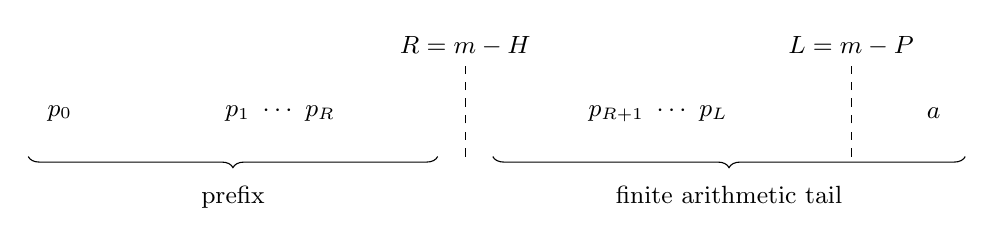
\begin{tikzpicture}[x=1cm,y=1cm,font=\small]
 \node at (0.4,0.45) {$p_0$};
 \node at (3.2,0.45) {$p_1\ \cdots\ p_R$};
 \node at (8,0.45) {$p_{R+1}\ \cdots\ p_L$};
 \node at (11.5,0.45) {$a$};
 \draw[dashed] (5.55,-0.1)--(5.55,1.05);
 \draw[dashed] (10.45,-0.1)--(10.45,1.05);
 \node[above] at (5.55,1.05) {$R=m-H$};
 \node[above] at (10.45,1.05) {$L=m-P$};
 \draw[decorate,decoration={brace,mirror,amplitude=4pt}]
       (0,-0.1)--(5.2,-0.1);
 \draw[decorate,decoration={brace,mirror,amplitude=4pt}]
       (5.9,-0.1)--(11.9,-0.1);
 \node[below] at (2.6,-0.35) {prefix};
 \node[below] at (8.9,-0.35) {finite arithmetic tail};
\end{tikzpicture}
\caption{The two cuts in a basic witness. We count $p_0$ by the prime
number theorem and approximate the $p_1,\ldots,p_R$ coordinates by volume.
The later primes and the smooth integer $a$ remain discrete.}
\label{fig:two-cuts}
\end{figure}

\begin{proposition}\label{prop:basic}
There is a set \(E_x\subseteq\mathcal V\cap[1,x]\) with
\[
 |E_x|\le\{\varepsilon_H+o_{x;H}(1)\}V(x)
\]
such that every preimage of every
\(v\in(\mathcal V\cap[1,x])\setminus E_x\) is
\(p_0\cdots p_La\) for a basic witness.  One may take
\[
 \varepsilon_H\ll
 \e^{-cP}+K_H\exp\{-\exp(cP\rho^{-P})\}.
\]
For every basic witness, putting \(w=p_{R+1}\cdots p_La\), we have
\begin{equation}\label{eq:cofactor-size}
 \begin{gathered}
 p_1\cdots p_La\le\exp((\log x)^{0.8}),\\
 \log w\le H\exp(0.62b_R)+\exp(2\widetilde b_L),
 \qquad w<p_R.
 \end{gathered}
\end{equation}
In particular \(w\) is bounded in terms of \(H\) alone, uniformly
in the phase.
\end{proposition}

We prove the proposition after the volume and smooth-cofactor estimates
below. Those estimates also prepare a second task: we shall retain the
shortened data \((p_0,\ldots,p_R,\varphi(w))\), then delete those
that fail the strict inequalities and normality conditions needed for
the collision argument. Coverage concerns \emph{values}; this later
deletion must count the distinct shortened tuples, including all tuples
that represent the same value.

\subsection{Simplex volume and concentration}
The coordinate scaling follows Ford's fundamental-simplex method
\cite[Lemma~3.2 and Corollary~3.3]{FordTotients2013}.
Our last adjacent coefficient is $a_1$ rather than $1$, so the exact
volume is slightly different from his; we derive it from the slacks
below. The recurrence estimate \eqref{eq:g-asymptotic} is Ford's
Lemma~3.7; his Remark~1 credits its streamlined proof to Lau's solution
of a recurrence problem \cite{FordLau2000}.

The next estimates turn sums over the allowed prime coordinates into
simplex volumes. We also bound the mass near a coordinate boundary or
a simplex face, so that removing these regions has a controlled cost.

\begin{lemma}\label{lem:simplex}
Let \(1\le j\le m\).  The true simplex \(S_j(\boldsymbol1)\) has volume \(G_j\).
Under its uniform volume measure the variables \(W_i=g_is_i/B\)
are uniform on \(\{W_i\ge0:\sum_{i=0}^jW_i=1\}\).
Moreover,
\[
 \operatorname{Vol}S_j(\boldsymbol\beta)
 \le G_j\prod_{r<j}\beta_r^{j-r}.
\]
Within \(S_j(\boldsymbol\beta)\), a specified slack \(s_t\) in an
interval of length \(D\) occupies at most a fraction \(jg_tD/B\)
of the volume.  A specified coordinate \(u_t\), \(1\le t\le j\),
in such an interval occupies at most \(jg_t\beta_tD/B\).
\end{lemma}

\begin{proof}
For the true simplex the triangular inversion is
\[
 u_i=\sum_{t=i}^j g_{t-i}s_t,\qquad
 B=\sum_{t=0}^j g_ts_t.
\]
The transformation from \(u_1,\ldots,u_j\) to \(s_1,\ldots,s_j\)
has determinant \(1\).  This proves the volume and distribution
statements.

Set \(K_i=\prod_{r<i}\beta_r\), \(K_0=1\).
The map \(u_i\mapsto u_i/K_i\) sends
\(S_j(\boldsymbol\beta)\) into \(S_j(\boldsymbol1)\), because
\(K_r\ge\beta_iK_i\) when \(r>i\).  Its inverse Jacobian is
\(\prod_{r<j}\beta_r^{j-r}\).

For the slice estimates, define
\(\gamma'_0=1\) and
\(\gamma'_t=\beta_t^{-1}\sum_{i<t}\gamma'_ia_{t-i}\).
Then \(0<\gamma'_t\le g_t\) and
\[
 \sum_{t=0}^j\gamma'_ts_t=\beta_0B.
\]
The marginal density of \(s_t\), under the uniform measure on this
simplex, is at most \(j\gamma'_t/(\beta_0B)\).
For the coordinate assertion, fix all other positive-index slacks.
The coordinate \(u_t\) is affine in \(s_t\) with slope \(1/\beta_t\).
Integrating first in this fiber and bounding by the full projection
volume gives the additional factor \(\beta_t\).
\end{proof}

The following concentration estimate will be used in Section~\ref{sec:limits}
to remove the prefix bands after replacing prime sums by volumes.
Write $z_+=\max\{z,0\}$.

\begin{lemma}\label{lem:concentration}
Fix \(\eta>0\).  There are constants \(C_\eta,c_\eta>0\) such that,
if \(Q\) is an integer with \(0\le Q<m\), \(j=m-Q\),
\(1\le i\le j\), and \(h_i\ge C_\eta(Q+1)\), then
uniform volume measure on \(S_j(\boldsymbol1)\) satisfies
\[
 \Pr(|u_i/b_i-1|>\eta)\le C_\eta\e^{-c_\eta h_i}.
\]
Also, for \(T\ge0\),
\[
 \Pr(u_j\ge T)=(1-g_jT/B)_+^j\le\e^{-jg_jT/B}.
\]
\end{lemma}

\begin{proof}
By \eqref{eq:g-asymptotic} and Lemma~\ref{lem:simplex},
\[
 \frac{u_i}{B\rho^i}
 =\sum_{t=i}^j(1+O(\rho^{t-i}))W_t.
\]
Represent \(W_t=E_t/\sum_{r=0}^jE_r\), where the \(E_t\) are
independent mean-one exponential variables.  The main numerator has
\(j-i+1=h_i-Q+1\) terms, and
\[
 \frac{(j-i+1)/(j+1)}{h_i/m}
 =1+O((Q+1)/h_i).
\]
Exponential moment bounds give exponentially small probabilities
for a fixed relative deviation of either the numerator or the
denominator.  The error numerator is bounded in absolute value by
\(C\sum_{r\ge0}\rho^rE_{i+r}\); this sum has a uniformly bounded
exponential moment, since
\(\prod_{r\ge0}(1-z\rho^r)^{-1}<\infty\) for \(0<z<1\).
Once \(h_i\ge C_\eta(Q+1)\), these three bounds give the first
assertion.  The second is the exact marginal tail of \(W_j\).
\end{proof}

\subsection{Prime boxes and smooth cofactors}
The use of reciprocal prime sums and enlarged coordinate boxes follows
Ford's Lemma~3.1 and the thickening arguments of his Section~3
\cite{FordTotients2013}. We record the quantitative bounds for our
simplexes, including the boundary errors needed for the tail unions.

We use unit boxes in the coordinates \(\log_2p_i\).
Mertens' theorem gives
\begin{equation}\label{eq:mertens-box}
 \sum_{b\le\log_2p<b+1}\frac1{p-1}=1+O(\e^{-b})
 \qquad(b\ge2).
\end{equation}
The replacement of \(1/p\) by \(1/(p-1)\) changes the sum by
\(O(\exp(-\exp b))\).  When the lower endpoints grow geometrically
backwards through the coordinates, multiplying
\eqref{eq:mertens-box} costs only a bounded factor; if their sum
of errors is small, it is the relative product error.

\begin{lemma}\label{lem:boxes}
Let \(0\le j\le L\).  Sum over primes \(p_1,\ldots,p_j\) whose
coordinates satisfy
\[
 0.9\widetilde b_i\le u_i\le1.1\widetilde b_i,\qquad
 (u_1,\ldots,u_j)\in S_j(\boldsymbol\xi).
\]
Then
\begin{equation}\label{eq:projected-mass}
 \sum_{p_1,\ldots,p_j}\prod_{i=1}^j\frac1{p_i-1}\ll G_m.
\end{equation}
Every unit box meeting this region lies in
\(S_j(\boldsymbol\beta)\), where, with a sufficiently large absolute
constant,
\begin{equation}\label{eq:box-enlargement}
 \beta_t=1+C\bigl(\e^{-h_t/40}+h_t^2\rho^{h_t}\bigr)
 \quad(0\le t<j),\qquad \beta_j=1.
\end{equation}
This enlargement has bounded volume cost.  Its coordinate scaling
factors through \(R\) differ from \(1\) by
\(O(\e^{-H/40}+H^2\rho^H)\).

There is also the following shell estimate in \(L\) coordinates.
Fix \(A>0\).  Among unit boxes meeting the displayed region, retain
those with a point satisfying, for some \(i\le R\), at least one of
these conditions:
\begin{enumerate}[label=(\roman*)]
\item \(i\ge1\) and \(u_i\) is within \(A\) of a coarse band endpoint;
\item the absolute value of
\(\xi_i u_i-\sum_{r=i+1}^L a_{r-i}u_r\) is at most \(Ah_i^2\);
\item \(\sum_{r=i+1}^L a_{r-i}u_r\ge(1-h_i^{-4})u_i\).
\end{enumerate}
The total volume of these boxes, and their total reciprocal-prime
weight, is
\begin{equation}\label{eq:boundary-mass}
 O_A(H^{-2}G_m).
\end{equation}
The same estimate holds when any subset of coordinates uses
reciprocal-prime measure and the others use Lebesgue measure.
For conditions (i)--(ii) alone, or for the region lost by replacing
the prefix coefficients \(\xi_i\), \(0\le i\le R\), with \(1\),
the stronger bound is
\[
 O_A\left(G_m\sum_{h\ge H}
       (h\e^{-h/40}+h^3\rho^h)\right).
\]
\end{lemma}

\begin{proof}
The band lower bounds are \(u_t\gg h_t\rho^{-h_t}\).
Changing each coordinate by at most \(1\) changes inequality \(t\)
by \(O(h_t^2)\).  These errors are absorbed by
\eqref{eq:box-enlargement}, including at \(t=0\), where \(u_0=B\)
is fixed.  The logarithm of its Jacobian upper bound is at most
\[
 C\sum_{h\ge P}h\bigl(\e^{-h/40}+h^2\rho^h\bigr)\ll1.
\]
Lemma~\ref{lem:simplex}, \eqref{eq:G-uniform}, and
\eqref{eq:mertens-box} prove \eqref{eq:projected-mass}.
The coordinate scaling factor is \(\prod_{t<i}\beta_t\), without
the Jacobian exponents; summing for \(h_t>h_i\ge H\) proves its
stated bound.

For the shells put \(h=h_i\).  Throughout a box meeting the bands,
\(u_i\ll b_i\).  Conditions (ii) and (iii), together with the unit
perturbations, put the enlarged slack in an interval starting at
zero of length at most
\[
 C_A\{b_i(h^{-4}+\e^{-h/40})+h^3\}.
\]
Here the \(h^3\) term includes
\(h^2\rho^hu_i=O(h^3)\).
Since \(Lg_i/B\ll\rho^h\), Lemma~\ref{lem:simplex} bounds the
relative volume by
\[
 C_A(h^{-3}+h\e^{-h/40}+h^3\rho^h).
\]
Condition (i), after expanding its interval by \(2\), costs only
\(O_A(\rho^h)\).  Sum these estimates over \(h\ge H\), and use
the bounded enlargement cost.  The prime-weight assertion follows
again from \eqref{eq:mertens-box}.
For the stronger assertion, omit \(h^{-4}\) from the slack interval.
Changing \(\xi_i\) to \(1\), for \(i\le R\), only removes points whose old slack is
between \(0\) and \((\xi_i-1)u_i\), which obey the same bound.
Finally every full unit box has uniformly bounded mass when an
arbitrary subset of its coordinates uses reciprocal-prime measure:
multiply the factors in \eqref{eq:mertens-box} for precisely that
subset.  This proves the mixed-measure assertion as well.
\end{proof}

\begin{lemma}\label{lem:smooth-tail}
Uniformly for \(Y\ge\exp(\exp2)\) and \(Z\ge0\),
\[
 \sum_{P^+(a)\le Y}\frac{a^{1/\log Y}}{\varphi(a)}\ll\log Y,
 \qquad
 \sum_{\substack{P^+(a)\le Y\\\log a>Z}}\frac1{\varphi(a)}
 \ll(\log Y)\exp(-Z/\log Y).
\]
In particular, with \(Y=\exp\exp(1.1\widetilde b_L)\),
\begin{equation}\label{eq:smooth-cost}
 \sum_{P^+(a)\le Y}\frac1{\varphi(a)}\le K_H,\qquad
 \sum_{\substack{P^+(a)\le Y\\\log a>\exp(2\widetilde b_L)}}
 \frac1{\varphi(a)}
 \le K_H\exp\{-\exp(cP\rho^{-P})\}.
\end{equation}
\end{lemma}

\begin{proof}
Put \(\sigma=1/\log Y\).  The Euler factor is
\[
 1+\frac{p^\sigma}{(p-1)(1-p^{\sigma-1})},
\]
whose logarithm is \(p^{-1+\sigma}+O(p^{-2+2\sigma})\), uniformly
in this range of \(\sigma\).  Partial summation gives
\(\sum_{p\le Y}(p^{-1+\sigma}-p^{-1})=O(1)\); hence the product
is \(O(\log Y)\).  Rankin's inequality gives the tail bound.
For the last assertion the exponent is
\[
 1.1\widetilde b_L-\exp(0.9\widetilde b_L),
\]
and \(\widetilde b_L\asymp P\rho^{-P}\).
\end{proof}

Combining Lemmas~\ref{lem:boxes} and \ref{lem:smooth-tail}, the shell
estimates remain valid after summing a smooth cofactor with weight
\(1/\varphi(a)\), at a cost of at most \(K_H\).
In particular their weighted mass is bounded by
\begin{equation}\label{eq:weighted-boundary}
 C K_HG_m\left\{H^{-2}+
       \sum_{h\ge H}(h\e^{-h/40}+h^3\rho^h)\right\}.
\end{equation}
The \(H^{-2}\) term is needed only for condition (iii).

\subsection{Coverage of the values}

\begin{proof}[Proof of Proposition~\ref{prop:basic}]
Take \(\eta=0.04\) in \eqref{eq:ford-bands}.  By
\eqref{eq:alpha-comparison}, its complementary bands imply the
coarse bands in \eqref{eq:basic}.  Apply
\eqref{eq:ford-simplex} as well.
Both conclusions hold for all preimages outside the union of their
exceptional sets.

We may also remove \(v\le x^{0.95}\) and \(\Omega(v)>5B\), at a
cost \(o(V(x))\).  For the latter, the elementary reciprocal moment
bound with \(z=1.9<2\) gives
\[
 \#\{v\le x:\Omega(v)>5B\}
 \le z^{-5B}x\sum_{r\le x}\frac{z^{\Omega(r)}}r
 \ll x\exp((z-5\log z)B)=o(x/\log x).
\]
The Euler product bounds the reciprocal sum by \(O((\log x)^z)\),
and \(z-5\log z<-1\).
For every preimage, \(\Omega(n)\le\Omega(\varphi(n))+1\le6B\).
The \(p_1\) band gives \(\log p_1\le(\log x)^{0.61}\), so
\[
 \log p_0\ge0.95\log x-6B(\log x)^{0.61}>0.9\log x.
\]

It remains to impose the size restriction on \(a\).  For any
preimage failing it, fix \(p_1,\ldots,p_L,a\).
The prime \(p_0\) is distinct from the others and from the factors
of \(a\).  Supermultiplicativity of \(\varphi\) gives
\[
 \varphi(p_0\cdots p_La)
 \ge(p_0-1)\varphi(a)\prod_{i=1}^L(p_i-1).
\]
The prime number theorem upper bound therefore gives at most
\[
 \frac{Cx}{\log x}\,
 \frac1{\varphi(a)\prod_{i=1}^L(p_i-1)}
\]
choices of \(p_0\); if the interval is nonempty its upper endpoint
is at least \(x^{0.9}\).  Sum the prefix by
Lemma~\ref{lem:boxes}, and the cofactor by
Lemma~\ref{lem:smooth-tail}.  This bounds all failing preimages,
and therefore all values having at least one such preimage.
It proves the exceptional-value assertion.

Finally \(b_{i+1}/b_i=(1-1/h_i)\rho\).
The bands and \eqref{eq:alpha-comparison} imply that the largest
double logarithm after index \(R\) is at most \(0.62b_R\).
There are \(H-P\le H\) such primes, proving the second line of
\eqref{eq:cofactor-size}.  Its right-hand side is smaller than
\(\exp(0.89b_R)<\log p_R\) for large \(H\), then large \(x\).
For the first line use the \(p_1\) bound and
\(L\ll\log B\), while the \(a\) bound depends only on \(H\).
\end{proof}

\subsection{Tuples and their discarded part}

For \(t=x\) or \(t=x/c\), where \(c>1\) is fixed, keep all
parameters formed from \(x\).  Let \(\mathcal T(t)\) be the set
of distinct tuples
\[
 \tau=(p_0,\ldots,p_R,d)
\]
admitting at least one basic witness with
\[
 d=\varphi(w),\qquad w=p_{R+1}\cdots p_La,\qquad
 d\prod_{i=0}^R(p_i-1)\le t.
\]
Each tuple represents a totient, because \(w<p_R\) makes its tail
coprime to its prefix.  Several witnesses may give the same tuple;
\(\mathcal T(t)\) counts that tuple once.

We next remove tuples for which the comparison argument might fail.
For each \(0\le i\le R\), put \(h=h_i\) and
\[
 J_i=\lceil30\log h\rceil,\qquad
 S_i=\exp\exp(b_i^{1/3}),\qquad
 z_i=\exp\exp(0.7b_{i+J_i}),
\]
and, for a basic witness, put
\[
 D_i=\varphi(p_{i+J_i+1}\cdots p_La).
\]
For large \(H\) these indices exist:
\(J_i<h_i/2\) and \(i+J_i<L\).
We call a tuple good if \emph{every} basic witness giving it satisfies,
for every \(0\le i\le R\),
\begin{equation}\label{eq:good-conditions}
 \begin{gathered}
 \sum_{r=i+1}^L a_{r-i}u_r\le(1-h_i^{-4})u_i,\\
 p_i,\ldots,p_{i+J_i}\text{ are }S_i\text{-normal},\\
 (p_i-1)\cdots(p_{i+J_i}-1)
 \text{ is squarefree on primes exceeding }z_i,\\
 \Omega(D_i)\le b_i/h_i^8 .
 \end{gathered}
\end{equation}
As before, the first condition uses \(u_0=B\).
Denote the good tuples by \(\mathcal G(t)\), and put
\(\mathcal D(t)=\mathcal T(t)\setminus\mathcal G(t)\).

\begin{proposition}\label{prop:discard}
For \(t=x\) and \(t=x/c\), with the same \(x\)-dependent parameters,
\[
 |\mathcal D(t)|
 \le\{\varepsilon_H+o_{x;H}(1)\}\frac{xG_m}{\log x}.
\]
One may take \(\varepsilon_H\ll K_HH^{-2}\).
For all the witnesses in \eqref{eq:good-conditions} we also have
\begin{equation}\label{eq:tail-cutoffs}
 P^+(D_i)<z_i,\qquad S_i<z_i,\qquad
 c h_i^{-20}\le b_{i+J_i}/b_i\le C h_i^{-18}.
\end{equation}
\end{proposition}

\begin{proof}
The last comparison follows from
\[
 \frac{b_{i+J_i}}{b_i}=(1-J_i/h_i)\rho^{J_i},
 \qquad 18<30\log(1/\rho)<20.
\]
It gives \(S_i<z_i\).  The next prime band has upper endpoint,
in double logarithms, less than \(0.7b_{i+J_i}\); all remaining
primes, including those in \(a\), are smaller.  Taking totients
cannot introduce a prime above this bound.  This proves
\eqref{eq:tail-cutoffs}.

A bad tuple has at least one failing full witness.  We bound the
number of these witnesses; this is an upper bound for the number of
bad tuples, regardless of witness multiplicity.
The prime-count upper bound for \(p_0\) contributes
\(Cx/\log x\), with the product of reciprocal factors for all
other variables.  The smooth \(a\)-sum contributes at most \(K_H\).
Failure of the first condition in \eqref{eq:good-conditions}
is covered by Lemma~\ref{lem:boxes}, condition (iii).
Its contribution is therefore \(O(K_HH^{-2}xG_m/\log x)\).

For the other conditions fix \(i\), write \(h=h_i\), \(b=b_i\),
and \(J=J_i\).  If \(i\ge1\), the reciprocal sum for the common
initial segment \(p_1,\ldots,p_{i-1}\) is \(O(G_m)\), by
\eqref{eq:projected-mass}.  All of \(p_i,\ldots,p_L\) are at most
\(\exp\exp(1.2b)\).  Their unrestricted reciprocal sums together
cost \(\exp(Ch^2)\), since there are at most \(h\) variables and
\(\log b=O(h)\).  For \(i=0\), omit \(p_0\) from these reciprocal
sums and use the same estimate at \(b=B\).

Partial summation of \eqref{eq:normal-primes} gives
\[
 \sum_{\substack{p\le\exp\exp(1.2b)\\
                   p\ {\rm not}\ S_i\text{-normal}}}\frac1{p-1}
 \ll(1+b)^6\e^{-b^{1/3}/6}
 \le\e^{-c b^{1/3}}.
\]
For a failure involving \(p_0\), apply
\eqref{eq:normal-primes} directly to its counting interval;
its upper endpoint has logarithm comparable with \(\log x\).
The normality failures thus contribute, relative to \(xG_m/\log x\),
at most
\begin{equation}\label{eq:normal-discard}
 K_H\sum_{h\ge H}\exp(Ch^2-cb(h)^{1/3}),
 \qquad b(h)=\alpha h\rho^{-h}.
\end{equation}
Polynomial factors from choosing an index are included in \(Ch^2\).

A square of a prime \(q>z_i\) in the shifted-prime product either
divides one shift twice or divides two different shifts.
For \(\ell=1,2\) and \(Z\ge2\), the elementary estimate
\[
 \sum_{\substack{p\le Z\\q^\ell\mid p-1}}\frac1{p-1}
 \le\frac{1+\log Z}{q^\ell}
\]
follows by summing over all positive multiples of \(q^\ell\).
If the shift is \(p_0-1\le T\), its integer count is at most
\(\lfloor T/q^\ell\rfloor\le T/q^\ell\).
Relative to prime counting this loses at most \(\log x=\e^b\)
when \(i=0\).  Both types of square therefore cost \(q^{-2}\),
up to \(\exp(Cb+Ch^2)\).  Summing over \(q>z_i\), their total
relative contribution is at most
\begin{equation}\label{eq:square-discard}
 K_H\sum_{h\ge H}
 \exp\{Ch^2+Cb(h)-\exp(c b(h)h^{-20})\}.
\end{equation}

Finally \(\Omega(\varphi(a))\ll\log a\le\e^{2\widetilde b_L}
=H^{o(1)}\), whereas \(b_i/h_i^8\) is exponentially large in
\(h_i\ge H\).  In the identity for \(D_i\), overlap between \(a\)
and the displayed primes can occur only at \(p_L\).
That overlap changes the sum of factor counts by
\(1-\Omega(p_L-1)\le0\).
Failure of the last condition in \eqref{eq:good-conditions}
therefore forces some \(i+J<j\le L\) to satisfy
\(\Omega(p_j-1)>b_i/(2h^9)\).
The Euler product gives
\[
 \sum_{n\le Z}\frac{(3/2)^{\Omega(n)}}n\ll(\log Z)^{3/2}.
\]
Using the band bound for \(p_j\), this exceptional reciprocal sum
is at most
\[
 \exp(Cb_{i+J}-cb_i/h^9)\le\exp(-c'b_i/h^9),
\]
because \(b_{i+J}\ll b_i h^{-18}\).
The resulting relative contribution is at most
\begin{equation}\label{eq:omega-discard}
 K_H\sum_{h\ge H}\exp(Ch^2-cb(h)/h^9).
\end{equation}
Each sum in \eqref{eq:normal-discard}--\eqref{eq:omega-discard}
decreases faster than every inverse power of \(H\), uniformly for
\(\alpha\) in its compact range.  Together with the thin-slack
bound, this proves the proposition.  Replacing the endpoint \(x\)
by \(x/c\) only decreases the witness sets, so the same bound holds
with unchanged parameters.
\end{proof}

The two cuts have now served different purposes.  The cut at \(L\)
keeps the smooth-cofactor cost at \(K_H=H^{o(1)}\); the earlier
cut at \(R\) supplies the summable \(H^{-2}\) loss and the much
stronger savings in the remaining discards.  Proposition~\ref{prop:basic}
controls exceptional \emph{values}, while
Proposition~\ref{prop:discard} controls exceptional \emph{tuples}.
Neither yet asserts uniqueness of a representation.  That is the
purpose of the comparison and collision arguments that follow.

\section{Comparing products of shifted primes}\label{sec:layers}

We next bound the number of ways that two ordered lists of primes can
give the same product of their shifts.  The largest prime factors of the
shifts lie in separated intervals.  We expose the factors one interval
at a time, starting with the smallest interval.  At each stage only two
or three simultaneous prime conditions are needed.  This keeps the
constants uniform when the number of intervals grows.

The layer decomposition and the comparison of dual factorizations
go back to Maier and Pomerance \cite[Section~3]{MaierPomerance1988}
and were developed further in Ford's proof of Lemma~5.1
\cite{FordTotients2013}. We prove the version needed here,
including its dependence on the number of layers.  In particular, we
assume squarefreeness of the whole product above the last cutoff;
squarefreeness of each individual shift would not suffice for our
factor-allocation estimate.

\subsection{A uniform sieve for two or three forms}

\begin{lemma}\label{lem:sieve}
There are absolute constants $C$ and $y_0$ with the following property.
Let $y\ge y_0$, put $B_y=\log_2 y$, and let $1\le A,A'\le y$ be
integers.  Consider either the two forms
\[
 n,\quad An+1,
\]
or the three forms
\[
 n,\quad An+1,\quad A'n+1,\qquad A\ne A'.
\]
Write $k=2$ or $3$, respectively, and let $\mathcal P$ be the set of
positive integers at which all the indicated forms are prime.  Then,
uniformly for $X\ge3$,
\begin{equation}\label{eq:sieve-count}
 \#(\mathcal P\cap[1,X])
 \le C\frac{X B_y^k}{(\log X)^k}.
\end{equation}
Moreover, uniformly for $3\le U\le Y$,
\begin{equation}\label{eq:sieve-reciprocal}
 \sum_{\substack{n\in\mathcal P\\U\le n\le Y}}\frac1n
 \le C\frac{B_y^k}{(\log U)^{k-1}}.
\end{equation}
The coefficients need not be bounded in terms of $X$ or $U$.
\end{lemma}

\begin{proof}
For primitive, distinct, admissible integral linear forms
$a_jn+b_j$ with positive leading coefficients and nonzero determinant
$\Delta$ as defined below, Ford's uniform upper sieve
\cite[Theorem~2.5]{FordSieve2023} gives
\begin{equation}\label{eq:sieve-determinant}
 \begin{gathered}
 \#\{1\le n\le X:a_jn+b_j\text{ prime for every }j\}
 \ll_k\frac{X}{(\log X)^k}
 \left(\frac{\Delta}{\varphi(\Delta)}\right)^k,\\
 \Delta=\left|\prod_j a_j
       \prod_{j<l}(a_jb_l-a_lb_j)\right|.
 \end{gathered}
\end{equation}
Here admissibility means that no prime divides the product of the
forms for every integer input; the implied constant depends only
on $k$, including when the coefficients vary.  For our forms,
primitivity is automatic, and the determinants are $A$ and
$AA'(A-A')$, up to sign.  They are nonzero and have absolute value at
most $y^3$.

If our forms are inadmissible, an offending prime is at most $k$, since
each primitive linear form has at most one root modulo that prime.
At every simultaneous-prime input one of the forms must equal this
prime.  Each such equality has at most one solution, so there are at
most $k$ inputs.  Their contribution is absorbed in
\eqref{eq:sieve-count}.

For admissible forms, the elementary estimate
\[
 \frac{d}{\varphi(d)}\ll\log_2(d+10)\qquad(d\ge1)
\]
and \eqref{eq:sieve-determinant} prove \eqref{eq:sieve-count}.
To recall its uniformity, split the product over prime divisors of
$d$ at $\log(d+10)$.  Mertens' product estimate bounds the first part
by $O(\log_2(d+10))$.  For the remaining part, use
$\sum_{p\mid d}\log p\le\log d$ to bound the sum of reciprocal
prime divisors, giving a bounded factor.  Since $k$ takes only the
values $2$ and $3$, all constants are absolute.

Finally, partial summation of \eqref{eq:sieve-count}, with the
coefficients fixed, gives
\[
 \sum_{\substack{n\in\mathcal P\\U\le n\le Y}}\frac1n
 \ll B_y^k\left(\frac1{(\log Y)^k}
       +\int_U^Y\frac{\dd t}{t(\log t)^k}\right)
 \ll\frac{B_y^k}{(\log U)^{k-1}}.
\]
This also includes a possible prime at the lower endpoint.
\end{proof}

\subsection{The comparison estimate}

For a positive integer $n$ and a real number $Z$, its part supported
above $Z$ means $\prod_{p^a\parallel n,\ p>Z}p^a$.  We use
$S$-normality as defined in Definition~\ref{def:normal}.

The key term in the bound below is the exponent of $\log y$.
In its application, a strict simplex inequality makes
the weighted cutoff sum plus its error smaller than $1$ by a
controlled amount.
The exponent is consequently smaller than $-1$; that extra saving
absorbs the other factors, even after recovering the tuple data hidden
in the smooth remainder. We need an estimate for ordered pairs with
multiplicity: a bound only on the number of values admitting a collision
would not control how many tuples lie over those values.

\begin{proposition}\label{prop:comparison}
There are absolute constants $C$ and $y_0$ such that the following
holds.  Let $y\ge y_0$, put $B_y=\log_2 y$, and let $b$ be an integer
with $1\le b\le B_y$.  Suppose that real cutoffs satisfy
\[
 Y_0=y,\qquad \e^\e\le S\le Y_b,
 \qquad Y_{j+1}<U_j<Y_j\quad(0\le j<b).
\]
Put
\[
 \nu_j=\frac{\log_2 Y_j}{B_y}\quad(0\le j\le b),
 \qquad
 \mu_j=\frac{\log_2 U_j}{B_y}\quad(0\le j<b),
 \qquad
 \delta=\sqrt{\frac{\log_2 S}{B_y}}.
\]
Fix a positive integer $D$ with $P^+(D)\le Y_b$ and a real $r\ge1$.
Let $N$ count the ordered tuples
\[
 (p_0,\ldots,p_{b-1},q_0,\ldots,q_{b-1},D')
\]
in which $D'$ is a positive integer and the following conditions hold:
\begin{enumerate}[label=\textup{(\roman*)}]
 \item The $p_j,q_j$ are $S$-normal primes, $p_j\ne q_j$, and
 \[
  U_j\le P^+(p_j-1),P^+(q_j-1)\le Y_j
  \qquad(0\le j<b).
 \]
 \item $P^+(D')\le Y_b$ and
 \[
  D\prod_{j=0}^{b-1}(p_j-1)
  =D'\prod_{j=0}^{b-1}(q_j-1)\le\frac yr.
 \]
 \item The common product in \textup{(ii)} is squarefree on primes
 greater than $Y_b$.
 \item The part of $p_0-1$ supported above $Y_1$ exceeds $\sqrt y$.
\end{enumerate}
Then
\begin{equation}\label{eq:comparison}
 \begin{split}
 N\le{}&\frac{y}{rD}(CB_y^6)^b(b+1)^{\Omega(D)}
       (\log Y_b)^{1+3b\log(b(b+1))}\\
 &\quad\times
 (\log y)^{-2+\sum_{j=1}^{b-1}a_j\nu_j+E_b},
 \end{split}
\end{equation}
where
\begin{equation}\label{eq:comparison-error}
 E_b=2\sum_{j=1}^{b-1}(\nu_j-\mu_j)
      +\delta\sum_{i=2}^b(i\log i+i).
\end{equation}
Here $a_j$ is as defined in \eqref{eq:aj}.  Empty sums are zero;
in particular, when $b=1$ the cutoff in
\textup{(iv)} is $Y_1=Y_b$.
\end{proposition}

\begin{proof}
We first describe the layers and the weighted summation that combines
them.  We then count the top layer, estimate a general lower layer,
and finally sum over the small prime factors.

\paragraph{The layer configurations.}
For $0\le i\le b$ and $0\le j<b$, let
\[
 s_{i,j}=\prod_{\substack{p^a\parallel p_j-1\\p\le Y_i}}p^a,
 \qquad
 s'_{i,j}=\prod_{\substack{p^a\parallel q_j-1\\p\le Y_i}}p^a.
\]
Restricting the equality in condition~\textup{(ii)} to primes at most
$Y_i$ gives the common product
\[
 s_i^\#=D\prod_{j=0}^{b-1}s_{i,j}
        =D'\prod_{j=0}^{b-1}s'_{i,j}.
\]
For $1\le i\le b$, put
\[
 t_{i,j}=\frac{s_{i-1,j}}{s_{i,j}},\qquad
 t'_{i,j}=\frac{s'_{i-1,j}}{s'_{i,j}},\qquad
 t_i^\#=\frac{s_{i-1}^\#}{s_i^\#}.
\]
Each $t_i^\#$ is squarefree and supported on $(Y_i,Y_{i-1}]$.
For $j\ge i$ the factors $t_{i,j}$ and $t'_{i,j}$ equal $1$, so
\begin{equation}\label{eq:layer-two-allocations}
 t_i^\#=\prod_{j=0}^{i-1}t_{i,j}
        =\prod_{j=0}^{i-1}t'_{i,j}.
\end{equation}
Thus a layer consists of two allocations of the same squarefree
integer among $i$ labeled slots.

Let $\mathcal C_i$ be the set of configurations
\[
 \sigma_i=(D',s_{i,0},\ldots,s_{i,b-1},
                   s'_{i,0},\ldots,s'_{i,b-1})
\]
arising from tuples counted by $N$.  Restriction of prime factors
maps $\mathcal C_{i-1}$ into $\mathcal C_i$; the two allocations in
\eqref{eq:layer-two-allocations} determine each extension uniquely.
Reconstructing a tuple from its small prime factors runs from
$\mathcal C_b$ back to $\mathcal C_0$; the weighted count below
sums in the opposite direction, starting with the top layer.
The original tuples are in bijection with $\mathcal C_0$, since
$p_j=s_{0,j}+1$ and $q_j=s'_{0,j}+1$.  For $i\ge2$ we will bound,
uniformly in $\sigma_i$, the reciprocal extension sum
\[
 \sum_{\substack{\sigma_{i-1}\in\mathcal C_{i-1}\\
                  \sigma_{i-1}\text{ restricts to }\sigma_i}}
       \frac1{t_i^\#}.
\]
This is the appropriate weight because
$1/s_{i-1}^\#=1/(s_i^\#t_i^\#)$.

Every configuration considered here extends to a genuine solution.
In particular, its partial common product is at most $y/r$, each
shift is at most $y$, and every fixed or conditional coefficient
used below is at most $y$.  When enlarging a sum for an upper bound,
we retain any necessary restriction on a conditional coefficient
until the corresponding sieve estimate has been applied.

\paragraph{The top layer.}
Only the zeroth shift can have a prime factor greater than $Y_1$.
Consequently $t_1^\#$ is the same part of $p_0-1$ and $q_0-1$,
and $t_1^\#>\sqrt y$.  Normality, applied with endpoint $p_0-1$,
gives
\[
 \Omega(p_0-1)
 \le B_y+\log_2 S+\sqrt{B_y\log_2 S}\le3B_y.
\]
Write $t_1^\#=t'Q$, with $Q=P^+(t_1^\#)$.  The weaker bound
$\Omega(t_1^\#)\le4B_y$ already gives
\[
 Q\ge y^{1/(8B_y)}.
\]
After $\sigma_1$ and $t'$ are fixed, the completed primes have the
forms $AQ+1,A'Q+1$.  Their inequality implies $A\ne A'$, which
is exactly the nonzero determinant condition for the three-form
sieve.  With
\[
 X=\frac{y}{r s_1^\#t'},
\]
a nonempty extension has $X\ge Q\ge y^{1/(8B_y)}$.
Lemma~\ref{lem:sieve} therefore bounds the number of $Q$ by
\[
 \ll\frac{X B_y^3}{(\log X)^3}
 \ll\frac{y}{r s_1^\#t'}\frac{B_y^6}{(\log y)^3}.
\]
The integer $t'$ is squarefree and supported on $(Y_1,y]$.
Mertens' estimate gives
\[
 \sum_{t'}\frac1{t'}
 \le\prod_{Y_1<p\le y}\left(1+\frac1p\right)
 \ll\frac{\log y}{\log Y_1}.
\]
It follows that, for each $\sigma_1$,
\begin{equation}\label{eq:top-layer}
 \#\{\sigma_0\text{ restricting to }\sigma_1\}
 \le CB_y^6\frac{y}{r s_1^\#}
       (\log y)^{-2-\nu_1}.
\end{equation}

\paragraph{The prime conditions in an intermediate layer.}
Fix $2\le i\le b$ and $\sigma_i$.  The last slot, of index
$i-1$, is complete after this layer.  Let $Q_1,Q_2$ be its largest
prime factors on the two sides; both lie in
$[U_{i-1},Y_{i-1}]$.

Suppose first that $Q_1=Q_2=Q$.  Remove the unique occurrence of
$Q$ from $t_i^\#$, and call the result $t$.  For fixed allocations
of $t$, the completed primes are $AQ+1,A'Q+1$ with $A\ne A'$.
Lemma~\ref{lem:sieve} gives
\begin{equation}\label{eq:shared-layer-prime}
 \sum_Q\frac1Q\ll\frac{B_y^3}{(\log U_{i-1})^2}.
\end{equation}

Now suppose $Q_1\ne Q_2$ and remove both, obtaining $t$.
In addition to its two allocations, fix the position of $Q_1$ on
the second side and of $Q_2$ on the first side.  There are at most
$i^2$ choices.  If neither prime lies in the opposite last slot,
the two completed prime conditions are
$AQ_1+1$ and $A'Q_2+1$; two applications of
\eqref{eq:sieve-reciprocal} with $k=2$ give
\begin{equation}\label{eq:distinct-layer-primes}
 \sum_{Q_1,Q_2}\frac1{Q_1Q_2}
 \ll\frac{B_y^4}{(\log U_{i-1})^2}.
\end{equation}
If $Q_2$ lies in the last slot on the first side, then $Q_2<Q_1$.
The prime $Q_1$ cannot lie in the last slot on the second side,
whose largest prime is $Q_2$.  The completed prime conditions are
now $AQ_2Q_1+1$ and $A'Q_2+1$.  First sum over $Q_1$ conditional
on $Q_2$, using the forms $Q_1,AQ_2Q_1+1$.  Feasibility ensures
$AQ_2\le y$, so the inner reciprocal sum is uniformly
$O(B_y^2/\log U_{i-1})$.  Only after this estimate do we enlarge
the range of $Q_2$ and apply the two-form bound to
$Q_2,A'Q_2+1$.  This proves \eqref{eq:distinct-layer-primes} again.
The reversed incidence is treated by reversing the order of
summation.  Both incidences cannot occur simultaneously, as they
would imply both $Q_1<Q_2$ and $Q_2<Q_1$.

\paragraph{Counting the allocations.}
Put $\Delta_i=\nu_{i-1}-\nu_i$.  Normality bounds the number of
prime factors of an individual shift in $(Y_i,Y_{i-1}]$ by
$(\Delta_i+\delta)B_y$.  Indeed, if the shift ends before
$Y_{i-1}$, apply normality only up to its endpoint; if it ends
before $Y_i$, the count is zero.  In either case the error is at
most $\sqrt{\log_2 S\,B_y}=\delta B_y$.
Only $i$ shifts contribute to this layer, and removing the
distinguished primes decreases the count.  Thus
\[
 \Omega(t)\le I_i:=i(\Delta_i+\delta)B_y.
\]
Since $t$ is squarefree, each of its prime factors chooses one of
$i$ slots on each side, giving at most $i^{2\Omega(t)}$ dual
allocations.  Write
\[
 M_i=\sum_{Y_i<p\le Y_{i-1}}\frac1p.
\]
Mertens' estimate gives $M_i\le\Delta_i B_y+O(1)$, uniformly in
the cutoffs.  Since $\delta B_y\ge\sqrt{B_y}$, increasing the
absolute threshold $y_0$ ensures
$M_i\le(\Delta_i+\delta)B_y$.  Hence
\begin{align}
 \sum_t\frac{i^{2\Omega(t)}}t
 &\le\sum_{n\le I_i}\frac{(i^2M_i)^n}{n!}
 \le i^{I_i}\exp(iM_i)\notag\\
 &\le\exp\bigl((i\log i+i)(\Delta_i+\delta)B_y\bigr).
 \label{eq:allocation-entropy}
\end{align}
The middle inequality follows by writing $i^{2n}=i^ni^n$,
using $i^n\le i^{I_i}$, and extending the remaining exponential
series.  It is valid without any lower bound on
$\Delta_i/\delta$.

Combining \eqref{eq:shared-layer-prime},
\eqref{eq:distinct-layer-primes}, and
\eqref{eq:allocation-entropy}, and using $i\le b\le B_y$ to
absorb the $i^2$ position choices, gives
\begin{equation}\label{eq:intermediate-layer}
 \sum_{\substack{\sigma_{i-1}\text{ restricting}\\
                  \text{to }\sigma_i}}\frac1{t_i^\#}
 \le CB_y^6
 (\log y)^{-2\mu_{i-1}+(i\log i+i)(\nu_{i-1}-\nu_i+\delta)}.
\end{equation}
The squarefree hypothesis was used both to remove a single
occurrence of each distinguished prime and to obtain the
factorial denominator in \eqref{eq:allocation-entropy}.

\paragraph{Multiplying the layer estimates.}
Starting from \eqref{eq:top-layer}, sum over $\mathcal C_1$.
For each subsequent layer use the exact weighted identity
\[
 \sum_{\sigma_{i-1}\in\mathcal C_{i-1}}\frac1{s_{i-1}^\#}
 =\sum_{\sigma_i\in\mathcal C_i}\frac1{s_i^\#}
   \sum_{\sigma_{i-1}\text{ restricting to }\sigma_i}
          \frac1{t_i^\#}.
\]
All bounds in \eqref{eq:intermediate-layer} are uniform in the
lower configuration.  Their constants therefore multiply to at
most $C^bB_y^{6b}$.  If $c_i=i\log i+i$, so that $c_1=1$, the
power of $\log y$ accumulated in this procedure is
\begin{align*}
 &-2-\nu_1+
   \sum_{i=2}^b\{-2\mu_{i-1}+c_i(\nu_{i-1}-\nu_i+\delta)\}\\
 &\qquad=-2+\sum_{j=1}^{b-1}a_j\nu_j
     +2\sum_{j=1}^{b-1}(\nu_j-\mu_j)
     +\delta\sum_{i=2}^b c_i-c_b\nu_b.
\end{align*}
Here $c_{j+1}-c_j-2=a_j$, including $j=1$.  The identity also
holds for $b=1$.  Discard the nonpositive final term
$-c_b\nu_b$.  It remains to bound
$\sum_{\sigma_b\in\mathcal C_b}1/s_b^\#$.

\paragraph{The smooth parts and repeated factors.}
Write $s=s_b^\#/D$ and $L_b=\log_2Y_b$.  For a fixed $s$, its
allocation among the $b$ left slots has at most $b^{\Omega(s)}$
possibilities.  The allocation of $sD$ among the $b$ right slots
and the additional slot $D'$ has at most
$(b+1)^{\Omega(sD)}$ possibilities.  These bounds allow prime
powers: assigning labeled copies of a repeated prime to slots
overcounts every possible distribution of its exponent.

Each left shift has largest prime factor above $Y_b$.  Its number
of prime factors at most $Y_b$ is bounded by normality as follows:
\[
 \Omega(p_j-1,1,Y_b)
 \le 2\log_2 S+(L_b-\log_2 S)
       +\sqrt{L_b\log_2 S}\le3L_b.
\]
If $S=Y_b$, the first normality inequality alone gives the same
bound.  Thus $\Omega(s)\le3bL_b$.  The ordinary smooth-number
Euler product, including all powers, now gives
\begin{align*}
 \sum_{\sigma_b\in\mathcal C_b}\frac1{s_b^\#}
 &\le\frac{(b+1)^{\Omega(D)}}D
   [b(b+1)]^{3bL_b}
   \sum_{P^+(s)\le Y_b}\frac1s\\
 &=\frac{(b+1)^{\Omega(D)}}D
   [b(b+1)]^{3bL_b}
   \prod_{p\le Y_b}\left(1-\frac1p\right)^{-1}\\
 &\ll\frac{(b+1)^{\Omega(D)}}D
   (\log Y_b)^{1+3b\log(b(b+1))}.
\end{align*}
No squarefreeness is assumed below $Y_b$.  Combining this estimate
with the layer bounds proves \eqref{eq:comparison}, after increasing
the absolute constant $C$.
\end{proof}

\begin{remark}\label{rem:comparison-uniformity}
The explicit error in \eqref{eq:comparison-error} satisfies
\[
 E_b=2\sum_{j=1}^{b-1}(\nu_j-\mu_j)
       +O\bigl(\delta b^2\log(2b)\bigr),
\]
and the smooth-factor exponent is $O(b\log(2b))$.  Thus all
dependence on a growing $b$ is displayed in
\eqref{eq:comparison}.  No restriction such as
$r\le y^{1/10}$ or $D\le y^{1/100}$ is needed: the large top
part supplies the lower bound for the actual sieve endpoint.
\end{remark}

\section{Uniqueness of the continuous prefix}\label{sec:collisions}

We now pass from representations to distinct totient values.  We retain the
tuple sets $\mathcal T(t)$, $\mathcal G(t)$ and $\mathcal D(t)$ of
Section~\ref{sec:extraction}: the first consists of the distinct tuples
$(p_0,\ldots,p_R,d)$ admitting a basic witness, the second consists of those
for which every basic witness satisfies \eqref{eq:good-conditions}, and
$\mathcal D(t)=\mathcal T(t)\setminus\mathcal G(t)$.  Their value map is
\[
 F(p_0,\ldots,p_R,d)=d\prod_{j=0}^R(p_j-1).
\]
The tail preimages of $d$ are not part of a tuple.  This distinction is
essential: we shall prove that almost every value has one such tuple,
while allowing several tail preimages.

\subsection{Counting pairs with the same value}
The alignment of largest factors and cancellation follow the argument
around (5.34)--(5.37) in Ford's Section~5 \cite{FordTotients2013}.
Here we count all ordered pairs of distinct tuples, including the data
inside both residual factors.
We first cancel the common prefix and align the large factors in the
remaining shifts. After applying the comparison estimate, we recover
the tuple coordinates inside the residual factors and then restore
the common prefix.

\begin{proposition}[Prefix collisions]\label{prop:collisions}
Fix $c>1$, and form all parameters from $x$, with $H$ fixed before $x$
tends to infinity.  For $t=x$ or $t=x/c$, let
\[
 K(t)=\#\{(\tau,\sigma)\in\mathcal G(t)^2:
             \tau\ne\sigma,\ F(\tau)=F(\sigma)\}.
\]
There is a quantity $\epsilon_H\to0$, independent of the phase, such that
\[
 K(t)\le\bigl(\epsilon_H+o_{x;H}(1)\bigr)
                   \frac{xG_m}{\log x}.
\]
The pairs counted here are ordered pairs of distinct tuples.
\end{proposition}

\begin{proof}
Choose one basic witness for each tuple under consideration.  All choices
satisfy \eqref{eq:good-conditions}, by the definition of $\mathcal G(t)$.
If two distinct tuples have the same value, some displayed prime differs:
equality of all the primes $p_0,\ldots,p_R$ would also force equality of
$d$.  Let $i$ be the first unequal prime index, and write $q_j$ for the
primes in the other witness.  Put
\[
 h=m-i,\qquad J=\lceil30\log h\rceil,\qquad
 z=z_i=\exp\exp(0.7b_{i+J}),\qquad S=S_i=\exp\exp(b_i^{1/3}).
\]
Thus $h\ge H$.  The residual integers in the good conditions are
\[
 D_i=\varphi(p_{i+J+1}\cdots p_La),\qquad
 D_i'=\varphi(q_{i+J+1}\cdots q_La').
\]
Canceling the common prefix leaves the identity
\begin{equation}\label{eq:suffix-identity}
 v^{(i)}=D_i\prod_{j=0}^{J}(p_{i+j}-1)
        =D_i'\prod_{j=0}^{J}(q_{i+j}-1).
\end{equation}
We will apply Proposition~\ref{prop:comparison} to this identity.  First
we verify its size and interval hypotheses; then we count all ways in
which its solutions can give tuple pairs.

\paragraph{Sizes of the suffix and its layers.}
For sufficiently large $H$, uniformly for $h\ge H$,
\begin{equation}\label{eq:collision-scales}
 b_i\asymp h\rho^{-h},\qquad
 \log b_i=O(h),\qquad
 c_1h^{-20}\le\frac{b_{i+J}}{b_i}
       =(1-J/h)\rho^J\le C_1h^{-18}.
\end{equation}
Indeed $30\lambda$ lies strictly between $18$ and $20$; the ceiling in
$J$ changes only constant factors.  In particular $J<h/2$ and
$i+J<L$.  The constants in this proof are independent of $H,x,i$ and the
phase, once $H$ and then $x$ are sufficiently large.

For $i=0$ set $y=x$.  For $i\ge1$ place $v^{(i)}$ in a dyadic interval
$(y/2,y]$.  The coarse bands in \eqref{eq:basic} imply that the logarithm
of the preimage suffix after $p_i$ is at most
\[
 h\exp(0.62b_i)+\exp(2\widetilde b_L).
\]
To see the first term, use
$1.1\widetilde b_{i+1}<0.62b_i$ for large $x$, and bound the number of
displayed factors by $h$.  The bound for $a$ gives the second term.
These quantities are negligible compared with
$\log p_i\ge\exp(0.88b_i)$.  Consequently, writing $B_y=\log_2y$,
\begin{equation}\label{eq:suffix-sizes}
 p_i,q_i\ge y^{0.9},\qquad
 0.88b_i\le B_y\le1.12b_i,\qquad u_i\le B_y+O(1).
\end{equation}
For $i=0$ the first inequality is part of the basic witness conditions,
and $B_y=b_0=u_0=B$ by convention.

Our target is a bound of the form
\[
 \frac{y}{\log y}\exp(-\kappa B_y/h^4)
\]
for the suffix pairs, with an absolute $\kappa>0$.
The strict simplex slack will supply the exponential saving.
Since $B_y\asymp b_i$, this saving can absorb the
$\exp(O(b_i\log h/h^8))$ cost of recovering tuple coordinates
inside $D_i$ and $D_i'$.

Let
\[
 \delta=\sqrt{\log_2S/B_y}\asymp b_i^{-1/3}.
\]
It follows from \eqref{eq:collision-scales} that $S<z$ and
$J\delta=o(h^{-20})$.  Normality gives
$\Omega(p_{i+j}-1),\Omega(q_{i+j}-1)\le4B_y$ for $0\le j\le J$.
For example, split the prime factors at $S$, apply the two normality
conditions, and use $p_{i+j}-1\le v^{(i)}\le y$.  If
\[
 A_j=P^+(p_{i+j}-1),\qquad A_j'=P^+(q_{i+j}-1),
\]
then
\begin{equation}\label{eq:largest-factor-band}
 \log_2A_j=u_{i+j}+O(\log b_i),\qquad
 \log_2A_j'=\log_2q_{i+j}+O(\log b_i).
\end{equation}
This follows from
$(p_{i+j}-1)\le A_j^{\Omega(p_{i+j}-1)}$ and the reverse bound
$A_j\le p_{i+j}-1$.  When $i=j=0$, the convention $u_0=B$
causes only an $O(1)$ difference from $\log_2p_0$, since
$x^{0.9}\le p_0\le x+1$.

The bands in \eqref{eq:largest-factor-band} are disjoint and decrease
with $j$.  Their smallest separation is a constant multiple of
$b_i h^{-20}$, which dominates the error $O(\log b_i)$.  All the $A_j,A_j'$
exceed $z$, whereas
\[
 P^+(D_i),P^+(D_i')<z.
\]
For the latter assertion, every prime in the residual preimage is at
most $p_{i+J+1}$ or $q_{i+J+1}$, and
$1.1\widetilde b_{i+J+1}<0.7b_{i+J}$; taking a totient cannot increase
the largest prime factor.  Repetitions of the last prime in $a$ or $a'$
do not affect this conclusion.

\paragraph{Aligning the largest factors on the two sides.}
We claim that
\begin{equation}\label{eq:factor-alignment}
 |\log_2 A_j-\log_2 A_j'|\le(2j+1)\delta B_y
                 \qquad(0\le j\le J).
\end{equation}
Suppose, for example, that $A_j>A_j'$, and put
$e=(\log_2 A_j-\log_2 A_j')/B_y$.  On the first side of
\eqref{eq:suffix-identity}, each of its first $j+1$ shifts contributes
at least $(e-\delta)B_y$ prime factors, with multiplicity, to
$(A_j',A_j]$.  On the other side only its first $j$ shifts can
contribute, each at most $(e+\delta)B_y$.  The later shifts have smaller
largest factors, and both residual integers are $z$-smooth.  The lower
endpoint exceeds $S$, so normality applies.  Equality of the two sides
therefore gives
\[
 (j+1)(e-\delta)\le j(e+\delta),
\]
which proves \eqref{eq:factor-alignment}.  Interchanging the sides
handles the other order.

Cancel any equal primes among the two lists in
\eqref{eq:suffix-identity}, and let $r$ be the product of their shifts.
The disjoint prime bands show that equality is possible only at the
same original index.  The index $i$ survives, since $p_i\ne q_i$.
Let $b\le J+1\le B_y$ be the length of the remaining lists.  Their corresponding
primes are unequal, as required by Proposition~\ref{prop:comparison}.

Set $Y_b=z$, $Y_0=y$ and $\log_2U_0=0.8B_y$.  At each remaining
positive index, choose an interval on a $\delta$-grid in normalized
double logarithms which contains the corresponding pair from
\eqref{eq:factor-alignment}.  Its width is $O(J\delta)$.  The intervals
remain strictly separated, because $J\delta=o(h^{-20})$.  Each lies
below height $0.8$, by \eqref{eq:suffix-sizes} and the upper bound
$u_{i+1}\le0.62b_i$.  At index zero,
\eqref{eq:suffix-sizes} and \eqref{eq:largest-factor-band} give largest
factors above height $0.9$.  Thus all the ordered-cutoff hypotheses of
Proposition~\ref{prop:comparison} hold.  If $b=1$, there are no positive
indices to grid and $Y_1=z$.

The part of $p_i-1$ supported on primes at most $Y_1$ has logarithm
at most $4B_y\log Y_1\le4B_y\exp(0.8B_y)$.  Since $p_i\ge y^{0.9}$,
the complementary part exceeds $\sqrt y$ for large $H$.  The whole
common product is squarefree above $Y_b$, by the good conditions;
canceling the equal shifts preserves this property.  This verifies
the last two hypotheses of Proposition~\ref{prop:comparison}.

Apply that proposition to the remaining lists with $D=D_i$, $D'=D_i'$
and the factor $r$ just canceled; their common product is at most $y/r$.
Write $\nu_k=\log_2Y_k/B_y$ and $\mu_k=\log_2U_k/B_y$ for the
normalized interval endpoints.

Write $j_1<\cdots<j_{b-1}$ for the surviving positive original
indices.  Since $j_k\ge k$ and $a_k\le a_{j_k}$, the grid intervals
and the strict slack condition in \eqref{eq:good-conditions} give
\begin{align}
 \sum_{k=1}^{b-1}a_k\nu_k
 &\le \frac{1}{B_y}\sum_{j=1}^{J}a_j u_{i+j}
                          +O(J^2\log(2J)\delta)\notag\\
 &\le1-h^{-4}+O(B_y^{-1}+J^2\log(2J)\delta).
 \label{eq:collision-slack}
\end{align}
Here $a_j$ is increasing and $\sum_{j\le J}a_j=O(J\log(2J))$.
The grid widths and the explicit $\delta$ term in
\eqref{eq:comparison} contribute another
$O(J^2\log(2J)\delta)=o(h^{-4})$ to its exponent of $\log y$.
Thus, for some absolute $\kappa>0$, its logarithmic factor is at most
\[
 (\log y)^{-1-\kappa h^{-4}}
 =\frac1{\log y}\exp(-\kappa B_y/h^4).
\]
It remains to show that the other factors and the recovery of tuple
coordinates use only a smaller part of this saving.

\paragraph{Recovering tuples and summing the remaining choices.}
The comparison estimate counts its displayed primes and its residual
integer $D_i'$.  We must also account for the tuple data forgotten
inside $D_i,D_i'$.  If $R\le i+J$, all displayed tuple primes are
already determined.  Their tail totient is
\[
 d=D_i\prod_{j=R+1}^{i+J}(p_j-1),
\]
and similarly on the other side, with an empty product when $R=i+J$.
If $R>i+J$, the missing tuple data give an ordered factorization
\begin{equation}\label{eq:residual-factorization}
 D_i=d\prod_{j=i+J+1}^{R}(p_j-1).
\end{equation}
There are at most $(h+1)^{\Omega(D_i)}$ such factorizations.  Indeed,
for any integer $n$, assigning its $\Omega(n)$ prime occurrences to
$k$ labeled slots bounds the number of ordered multiplicative
factorizations into $k$ factors by $k^{\Omega(n)}$.  Once a factor
$p_j-1$ is fixed, $p_j$ is fixed as well.  This argument also covers
repeated prime factors.  Consequently the two missing tails cost at most
\begin{equation}\label{eq:tuple-recovery-cost}
 (h+1)^{\Omega(D_i)+\Omega(D_i')}
       \le\exp\{2b_i\log(h+1)/h^8\}.
\end{equation}
The factorizations in \eqref{eq:residual-factorization} are exact:
the primes up to $R$ are distinct and the remaining preimage tail is
smaller than $p_R$, by \eqref{eq:cofactor-size}.  All repetitions inside
that tail are kept in its totient $d$.

We now sum the comparison bound over the canceled primes, the grids,
and $D_i$.  The canceled index sets contribute at most $2^{J+1}$.
Each canceled prime has reciprocal shift sum $O(b_i)$ by Mertens'
theorem.  The number of grid choices is at most
$(C/\delta)^{2(J+1)}$.  Thus their total cost, including the factors
$(CB_y^6)^b$ in \eqref{eq:comparison}, is $\exp(O(h^2))$.
For the residual integer, the finite Euler product gives
\[
 \sum_{P^+(D)\le z}\frac1D\ll\log z.
\]
Before enlarging this sum we use the good-condition bounds
$\Omega(D_i),\Omega(D_i')\le b_i/h^8$ in both
\eqref{eq:tuple-recovery-cost} and the factor $(b+1)^{\Omega(D_i)}$
of the comparison estimate.

The logarithm of all the remaining costs, apart from the factor
$y/(\log y)$ and the saving from \eqref{eq:collision-slack}, is at most
\begin{equation}\label{eq:collision-costs}
 O(h^2)+O\left(\frac{b_i\log h}{h^8}\right)
       +O\left(\frac{b_i\log h\log\log(3h)}{h^{18}}\right)
       =o\left(\frac{b_i}{h^4}\right).
\end{equation}
The last term uses
$\log_2z\ll b_i h^{-18}$ to bound the factor
$(\log Y_b)^{1+3b\log(b(b+1))}$ in \eqref{eq:comparison}, as well
as the sum over $D_i$.  All little-oh estimates here are uniform for
$h\ge H$ as $H\to\infty$, because $b_i\asymp h\rho^{-h}$.
We have therefore obtained, for some absolute $c_2>0$,
\begin{equation}\label{eq:suffix-pair-count}
 \#\{\text{ordered suffix tuple pairs with }y/2<v^{(i)}\le y\}
 \ll\frac{y}{\log y}\exp\{-c_2B_y/h^4\}.
\end{equation}
For $i=0$ the same expression bounds all the pairs with first unequal
index zero, using $y=x$.  Choosing one witness for each tuple has not
introduced multiplicity into the desired count: comparison data and
the factorizations just counted determine each ordered pair of tuples.

\paragraph{Summing suffixes and restoring the common prefix.}
For $i\ge1$ the required sum over suffix pairs is weighted by
$1/v^{(i)}$.  A dyadic interval in \eqref{eq:suffix-pair-count}
contributes at most
\[
 \frac{C}{\log y}\exp\{-c_2\log_2y/h^4\}.
\]
Writing the dyadic endpoints as $y=2^n$, and comparing the sum with
an integral, gives
\begin{align}
 \sum_{\text{suffix pairs}}\frac1{v^{(i)}}
 &\ll\sum_{\log(n\log2)\ge0.88b_i-O(1)}
       \frac{\exp\{-c_2\log(n\log2)/h^4\}}{n\log2}\notag\\
 &\ll\int_{0.88b_i-O(1)}^\infty\exp(-c_2u/h^4)\,\dd u
  \ll h^4\exp(-c_3b_i/h^4).
 \label{eq:dyadic-suffix-mass}
\end{align}
In this change of variable, $u=\log(n\log2)$, the factor
$1/\log y$ exactly compensates for the density of dyadic endpoints.
In particular, no factor of order $\exp(b_i)$ is lost.

For fixed suffix data and common primes $p_1,\ldots,p_{i-1}$, the
number of possible $p_0$ is at most
\[
 \frac{Cx}{\log x}\,
 \frac1{v^{(i)}\prod_{j=1}^{i-1}(p_j-1)}.
\]
Indeed the upper endpoint for $p_0$ is
$1+x/(v^{(i)}\prod_{j=1}^{i-1}(p_j-1))$; if the range is nonempty,
its restriction $p_0\ge x^{0.9}$ makes its logarithm comparable to
$\log x$, so the prime number theorem gives this upper bound.
The projected-prefix estimate \eqref{eq:projected-mass} and
\eqref{eq:dyadic-suffix-mass} now show that the contribution for this
$i$ is at most
\[
 \frac{CxG_m}{\log x}\,h^4\exp(-c_3b_i/h^4).
\]
This also applies to the empty projected prefix when $i=1$.
Summing over $h\ge H$ yields the convergent tail
\[
 C\sum_{h\ge H}h^4\exp\{-c_4\rho^{-h}/h^3\}\longrightarrow0.
\]
For $i=0$, \eqref{eq:suffix-pair-count} gives
$O((x/\log x)\exp\{-c_2B/m^4\})$, which is
$o(xG_m/\log x)$.  This proves the proposition, uniformly for both
endpoints $t$.
\end{proof}

\subsection{From tuples to values and least preimages}

The following elementary lemma keeps track of exceptional tuples as
well as exceptional values.  This is needed because a small set of
values could otherwise carry many representations.

\begin{lemma}[Finite-map counting]\label{lem:finite-map}
Let $T$ and $W$ be finite sets, let $F:T\to W$, and write
$T=G\sqcup D$.  Suppose that every element of $W\setminus E$ is
in $F(T)$, where $E\subset W$.  For $w\in W$ put
$r_w=|G\cap F^{-1}(w)|$, and let
\[
 K=\sum_{w\in W}r_w(r_w-1).
\]
Then
\[
 -|E|\le |T|-|W|\le |D|+K/2.
\]
Moreover, with
$E^*=E\cup F(D)\cup\{w:r_w\ge2\}$, one has
\[
 |E^*|\le|E|+|D|+K/2,\qquad
 |F^{-1}(E^*)|\le|E|+2|D|+K.
\]
The restriction of $F$ to $T\setminus F^{-1}(E^*)$ is a bijection
onto $W\setminus E^*$.
\end{lemma}

\begin{proof}
Coverage gives the lower bound.  For every positive integer $r$,
$r-1\le r(r-1)/2$, and hence
\[
 |G|-|F(G)|\le K/2.
\]
Adding the at most $|D|$ remaining elements proves the upper bound.
There are at most $K/2$ fibers with $r_w\ge2$, which proves the
bound for $|E^*|$.  Also
\[
 \sum_{w\in E^*}r_w\le|E^*|+K/2,
\]
by $r\le1+r(r-1)/2$ for integers $r\ge0$.  Adding the elements of
$D$ proves the second bound.  Outside $E^*$ coverage, absence of
discarded elements, and $r_w\le1$ give exactly one preimage under $F$.
\end{proof}

\begin{proposition}[A common prefix for all preimages]\label{prop:unique-prefix}
For $t=x$ or $t=x/c$, with the same parameters formed from $x$,
\begin{equation}\label{eq:tuple-cardinality}
 \bigl|\,|\mathcal T(t)|-V(t)\,\bigr|
       \le\bigl(\epsilon_H+o_{x;H}(1)\bigr)\frac{xG_m}{\log x},
 \qquad\epsilon_H\longrightarrow0.
\end{equation}
There is a set $E^*(t)\subset\mathcal V\cap[1,t]$ for which both
$|E^*(t)|$ and the number of tuples in $\mathcal T(t)$ with values in
$E^*(t)$ are at most
$(\epsilon_H+o_{x;H}(1))xG_m/\log x$, after enlarging $\epsilon_H$.
For every $v\in(\mathcal V\cap[1,t])\setminus E^*(t)$ there is a unique tuple
$(p_0,\ldots,p_R,d)\in\mathcal T(t)$ of value $v$, and every preimage
of $v$ has this prefix and a remaining factor of totient $d$.
In particular,
\begin{equation}\label{eq:least-factorization}
 \ell(v)=p_0\cdots p_R\ell(d).
\end{equation}
\end{proposition}

\begin{proof}
Apply Lemma~\ref{lem:finite-map} with $T=\mathcal T(t)$,
$G=\mathcal G(t)$, $D=\mathcal D(t)$ and
$W=\mathcal V\cap[1,t]$.  Let $E$ be the exceptional values in
Proposition~\ref{prop:basic}, restricted to $[1,t]$.  Every preimage
of each $v\notin E$ is basic, so it induces an element of $T$.
The size of $E$ is negligible on the scale $xG_m/\log x$, by
\eqref{eq:ford-scale}; Proposition~\ref{prop:discard} gives the same
bound for $|D|$, and Proposition~\ref{prop:collisions} gives it for
$K$.  The counting conclusions therefore follow from the lemma.

Fix $v\notin E^*(t)$.  Every preimage is basic and so induces a tuple
in $T$.  It cannot induce a tuple in $D$, since $v\notin F(D)$.
The remaining tuple is unique.  Thus, writing $Q=p_0\cdots p_R$,
every preimage of $v$ has the form $Qz$, where $\varphi(z)=d$.
It follows that every such preimage is at least $Q\ell(d)$.

For the reverse inequality choose one basic witness with tail $w$.
The deterministic size bound \eqref{eq:cofactor-size} gives
$\ell(d)\le w<p_R$.  The prefix primes are distinct, so
$\gcd(Q,\ell(d))=1$ and
\[
 \varphi(Q\ell(d))=\varphi(Q)\varphi(\ell(d))
                 =d\prod_{j=0}^R(p_j-1)=v.
\]
Hence $\ell(v)\le Q\ell(d)$, proving \eqref{eq:least-factorization}.
\end{proof}

The universal quantifier on preimages in Proposition~\ref{prop:basic}
is used only after the counting argument, to obtain the common-prefix
statement and \eqref{eq:least-factorization}.  A single basic preimage
would give the upper bound for $\ell(v)$ but would not give the reverse
inequality.

\section{The arithmetic coefficient and the limiting formula}
\label{sec:limits}

The preceding sections reduce the count of values to distinct tuples with
a common long prime prefix.  We now sum over the largest prime and replace
the remaining prefix by a volume.  The shorter tail stays discrete: its
different witnesses are combined by a union before taking that volume.
Throughout this section, $H$ is fixed first, $x$ tends to infinity next,
and $H$ tends to infinity last.  In particular, $P=\lfloor\log\log H\rfloor$,
$R=m-H$, and $L=m-P$ always refer to the two cuts in \eqref{eq:cuts}.

\subsection{Summing over the largest prime}

Let $\mathcal D_H(x)$ be the set of distinct data
$(d,p_1,\ldots,p_R)$ for which there are primes
$p_{R+1},\ldots,p_L$ and a positive integer $a$ satisfying
the basic conditions \eqref{eq:basic} with $p_0$ omitted, and
\[
 d=\varphi(w),\qquad w=p_{R+1}\cdots p_La.
\]
The convention $u_0=B$ is retained in these conditions.  Thus the
inequality with index zero is a condition on the displayed data and
their witness, independent of the eventual choice of $p_0$.
For any function $f:[1,\infty)\to[0,1]$, define
\begin{equation}
 M_f(x;H)=
 \sum_{(d,p_1,\ldots,p_R)\in\mathcal D_H(x)}
 \frac{f(\ell(d)/d)}{d\prod_{i=1}^R(p_i-1)}.
 \label{eq:mass}
\end{equation}
Each datum is included once, regardless of its number of witnesses.
The function $f=1$ makes the least-preimage ratio irrelevant to this
definition.

We use $K_H=\exp(CP\rho^{-P})=H^{o(1)}$, allowing the absolute constant
$C$ to increase in upper bounds.  Summing over witnesses, the totient
inequality
\begin{equation}
 \frac{1}{\varphi(p_{R+1}\cdots p_La)}
 \le \frac{1}{\varphi(a)}
       \prod_{i=R+1}^L\frac{1}{p_i-1}
 \label{eq:tail-reciprocal-majorant}
\end{equation}
and Lemma~\ref{lem:boxes} give
\begin{equation}
 0\le M_f(x;H)\le M_1(x;H)\ll K_HG_m.
 \label{eq:mass-upper}
\end{equation}
Indeed, the reciprocal sum for the full $L$ prime coordinates is
$O(G_m)$ by \eqref{eq:projected-mass}, while the unrestricted reciprocal
sum for the allowed smooth cofactor is $O(K_H)$ by
\eqref{eq:smooth-cost}.  The inequality in
\eqref{eq:tail-reciprocal-majorant}, rather than an equality, also
covers the possibility that $p_L$ divides $a$.

\begin{proposition}[The unweighted prime sum]
\label{prop:mass}
For each fixed $c>1$, both $t=x$ and $t=x/c$ satisfy
\begin{equation}
 V(t)=\frac{t}{\log x}
 \bigl(M_1(x;H)+E_H(t;x)G_m\bigr),
 \qquad
 \lim_{H\to\infty}\limsup_{x\to\infty}
 \max_{t\in\{x,x/c\}}|E_H(t;x)|=0.
 \label{eq:mass-count}
\end{equation}
All parameters in the two formulas are formed from the same $x$.
\end{proposition}

\begin{proof}
For fixed data in $\mathcal D_H(x)$ put
\[
 D=d\prod_{i=1}^R(p_i-1).
\]
Since $d\le w$, the deterministic bound \eqref{eq:cofactor-size}
implies
\[
 1\le D\le p_1\cdots p_La\le\exp((\log x)^{0.8}).
\]
The possible largest primes are precisely
$x^{0.9}\le p_0\le 1+t/D$.  The remaining prime factors are smaller
than $x^{0.9}$ for large $x$, so this choice introduces neither a
repeated prefix prime nor another ordering condition.  The endpoints
$t/D$ lie uniformly in $[x^{1-o(1)}/c,x]$.  The prime number theorem,
with $\log(t/D)=\log x+o(\log x)$ uniformly, therefore gives
\[
 \#\{p_0:x^{0.9}\le p_0\le1+t/D\}
 =\frac{t}{D\log x}\bigl(1+o_{x\to\infty;H,c}(1)\bigr).
\]
The lower cutoff costs a relative
$O(x^{-0.1+o(1)})$, uniformly in the data.  Summing this formula and
using \eqref{eq:mass-upper} counts $\mathcal T(t)$ with main term
$tM_1/\log x$ and error $o_{x\to\infty;H,c}(xG_m/\log x)$.
Proposition~\ref{prop:unique-prefix} replaces $\#\mathcal T(t)$ by
$V(t)$ with an error whose normalized iterated limit is zero.  Since
$t$ is either $x$ or $x/c$, this proves \eqref{eq:mass-count}.
\end{proof}

The common mass in Proposition~\ref{prop:mass} already gives the
fixed-scaling conclusion. Its proof does not require identifying that
mass with the arithmetic coefficient.

\begin{corollary}[Fixed scaling]\label{cor:fixed-scaling}
For every fixed real \(c>0\),
\[
 \frac{V(cx)}{V(x)}\longrightarrow c.
\]
\end{corollary}

\begin{proof}
First let \(c>1\). Apply Proposition~\ref{prop:mass} at \(t=x\)
and \(t=x/c\), using the same \(M_1(x;H)\) and \(G_m(x)\).
Subtracting gives
\[
 \frac{(V(x)-cV(x/c))\log x}{xG_m}
 =E_H(x;x)-E_H(x/c;x).
\]
Ford's estimate \eqref{eq:ford-scale} supplies a positive constant
\(c_-\) with \(V(x)\log x/(xG_m)\ge c_-\) for large \(x\).
Consequently
\[
 \limsup_{x\to\infty}
 \left|1-\frac{cV(x/c)}{V(x)}\right|
 \le\frac1{c_-}\limsup_{x\to\infty}
       \bigl(|E_H(x;x)|+|E_H(x/c;x)|\bigr).
\]
Let \(H\) tend to infinity and then replace \(x\) by \(cx\) to
obtain the assertion. This also covers arguments at which
\(m(x)\) and \(m(x/c)\) differ: the latter integer never enters
the comparison. Neither continuity of the phase coefficient nor
matching values at the ends of the phase interval is required.

The case \(c=1\) is immediate. If \(0<c<1\), apply the result
just proved to the multiplier \(1/c>1\) and the argument
\(y=cx\); taking reciprocals gives the stated limit.
\end{proof}

\subsection{A finite tail and a continuous prefix}

The phase-dependent witness set in \eqref{eq:AH} changes with the
phase, but for fixed $H$ all its members belong to one finite set.
This observation will permit uniform limits without any continuity
assumption.

\begin{lemma}[Uniformly finite tail data]
\label{lem:finite-tail-data}
For each sufficiently large fixed $H$, the union of all
$\mathcal W_{H,s}(d)$, over $0\le s<1$ and all $d$, is finite.
All its prime and integer coordinates, and all its totient values,
have explicit bounds depending only on $H$.  Uniformly over these
data,
\begin{equation}
 0\le D(h,\eta)\ll_H\log(2h)\qquad(h\ge H).
 \label{eq:tail-D-bound}
\end{equation}
\end{lemma}

\begin{proof}
Write $a_*=\lambda/\rho$, so that
$\lambda\le\alpha_s<a_*$.  Let
\[
 q_H=\left\lceil\exp\exp(1.1a_*H\rho^{-H})\right\rceil,
 \qquad
 A_H^*=\left\lceil\exp\exp(2a_*P\rho^{-P})\right\rceil.
\]
Every witness belongs to the finite set
$\{1,\ldots,q_H\}^{H-P}\times\{1,\ldots,A_H^*\}$.
Its corresponding integer $w$ and totient $d$ satisfy
$d\le w\le A_H^*q_H^{H-P}$.  These bounds do not involve $x$ or $s$.
Finally,
$a_j=\int_j^{j+1}\log t\,\dd t\le\log(j+1)$, so the definition
\eqref{eq:tail-D} and the bounded tail coordinates give
\eqref{eq:tail-D-bound}.
\end{proof}

For $s=\theta(x)$ and $\eta\in\mathcal W_{H,s}(d)$, define
the region $\mathcal K_\eta\subset\mathbb R^R$ by $u_0=B$ and
\begin{equation}
 u_i-\sum_{r=i+1}^Ra_{r-i}u_r\ge D(m-i,\eta)
 \qquad(0\le i\le R).
 \label{eq:prefix-region}
\end{equation}
These inequalities imply $u_i\ge0$.  The coordinates $u_i$ here are
real; the coarse prime bands have been removed.  We write
$\operatorname{Vol}_R$ for $R$-dimensional Lebesgue measure.

\begin{lemma}[The volume of the witness union]
\label{lem:tail-volume}
There are numbers $\delta_H\to0$ such that, uniformly for
$f:[1,\infty)\to[0,1]$,
\begin{equation}
 \limsup_{x\to\infty}
 \left|\frac{M_f(x;H)}{G_m}
 -\frac1{G_m}\sum_{d:\mathcal W_{H,\theta}(d)\ne\varnothing}
 \frac{f(\ell(d)/d)}d
 \operatorname{Vol}_R
 \bigcup_{\eta\in\mathcal W_{H,\theta}(d)}\mathcal K_\eta
 \right|\le\delta_H.
 \label{eq:mass-volume}
\end{equation}
Moreover, for every nonempty finite
$T\subseteq\mathcal W_{H,\theta}(d)$,
\begin{equation}
 \operatorname{Vol}_R\bigcap_{\eta\in T}\mathcal K_\eta
 =G_R\left(1-\frac1B\sum_{h=H}^m g_{m-h}
       \max_{\eta\in T}D(h,\eta)\right)_+^R.
 \label{eq:intersection-volume}
\end{equation}
Here $z_+=\max(z,0)$.
\end{lemma}

\begin{proof}
An intersection imposes the largest of the witness thresholds at each
slack coordinate.

\paragraph{Intersection volumes.}
Set $C_i=\max_{\eta\in T}D(m-i,\eta)$ and introduce the prefix
slacks
\[
 t_i=u_i-\sum_{r=i+1}^Ra_{r-i}u_r\qquad(0\le i\le R).
\]
Lemma~\ref{lem:simplex} gives
$\sum_{i=0}^Rg_it_i=B$, and the substitution from
$(u_1,\ldots,u_R)$ to $(t_1,\ldots,t_R)$ has determinant one.
The intersection is $t_i\ge C_i$ for every $i$, including $i=0$.
Translation by $C_i$ leaves a simplex of available size
$B-\sum_i g_iC_i$. Its volume is
\[
 \frac{(B-\sum_{i=0}^Rg_iC_i)_+^R}
 {R!\prod_{i=1}^Rg_i},
\]
which proves \eqref{eq:intersection-volume} after putting $h=m-i$.
It remains to compare the volume of the union with the prime mass.

\paragraph{From primes to volume.}
Identify $Q_h=p_{m-h}$ for $P\le h<H$.  These are exactly the
primes with indices $R+1,\ldots,L$.  For fixed tail witness $\eta$,
the original prefix conditions are its coarse bands together with
\begin{equation}
 \xi_i u_i-\sum_{r=i+1}^Ra_{r-i}u_r\ge D(m-i,\eta)
 \qquad(0\le i\le R).
 \label{eq:perturbed-prefix-region}
\end{equation}
Taking the union over $\eta\in\mathcal W_{H,\theta}(d)$ is essential:
a prime prefix with several witnesses contributes just once to
\eqref{eq:mass}.

First replace the reciprocal prime sum by the volume of this union
with its bands and its $\xi_i$.  In a unit box wholly contained in
the union, the product of the prime reciprocal
sums differs from its volume by a relative
$O(\sum_{i=1}^R e^{-c b_i})=O(e^{-c' b_R})$, by
Lemma~\ref{lem:boxes}.  The geometric growth of $b_i$ as $i$
decreases makes this estimate independent of $R$.  Both the total
mass and the total volume before this replacement are
$O(K_HG_m)$, by summing over witnesses as in
\eqref{eq:tail-reciprocal-majorant}.

If a unit box meets the union without being contained in it,
choose a witness whose region meets the box.  That witness's
region does not contain the box.  Consequently the box lies in
a shell at a prefix band endpoint, or within $O(h_i^2)$ of equality
in one of \eqref{eq:perturbed-prefix-region}.  For an upper bound,
sum these shells over witnesses using
\eqref{eq:tail-reciprocal-majorant}.  Thicken the discrete tail
coordinates into unit boxes as well and sum $1/\varphi(a)$ at a
cost $O(K_H)$.  The resulting full $L$-coordinate boxes are covered
by the shell bounds of Lemma~\ref{lem:boxes} and
Proposition~\ref{prop:discard}.  Their contribution is $o_H(1)G_m$.
More explicitly, the slice coefficient for an index with $h=m-i$
is $Lg_i/B\ll\rho^h$.  Summing the shell bounds therefore costs
at most
\[
 O\!\left(K_H\sum_{h\ge H}
       (h e^{-h/40}+h^3\rho^h)\right)G_m.
\]
The broader $O(K_HH^{-2})G_m$ shell estimate in
Proposition~\ref{prop:discard} also suffices.

\paragraph{Removing the slack perturbation.}
Replace $\xi_i$ by $1$ for $i\le R$, retaining the bands.
The removed region lies in a shell of thickness
$O(e^{-h_i/40}b_i)$, with the same box-thickening errors.
Its normalized contribution is at most
\[
 O\!\left(K_H\sum_{h\ge H}
       (h e^{-h/40}+h^3\rho^h)\right)=o_H(1).
\]
Both shell estimates are valid for the union because upper bounds
may sum over witnesses, while $0\le f\le1$.

\paragraph{Removing the prefix bands.}
For every point satisfying
the now unperturbed prefix inequalities, recurrence iteration gives
\begin{equation}
 u_i\ge g_{R+1-i}v_{H-1}\gg H\rho^{-h_i}
 \qquad(0\le i\le R),
 \label{eq:unbanded-prefix-lower}
\end{equation}
where $v_{H-1}=\log_2Q_{H-1}$.  To see this, retain the contribution
of the first tail coordinate in each prefix inequality, discard
the other nonnegative tail contributions, and apply the recurrence
for $g$.  The tail band for $v_{H-1}$ and
\eqref{eq:g-asymptotic} give the displayed lower bound.
Thickening the $H-P$ tail coordinates changes inequality $i$ by
$O(H\log(h_i+1))$. The enlargement term
$C h_i^2\rho^{h_i}u_i$ is at least a constant times $CHh_i^2$,
so it absorbs this error. Together with the retained tail bands,
this places the full region inside the enlarged simplex of
Lemma~\ref{lem:boxes}.

To sum these regions without a factor for the number of witnesses,
use \eqref{eq:tail-reciprocal-majorant} and first fix $a$. Partition
the tail coordinates into half-open unit boxes
$\mathcal C=\prod_{h=P}^{H-1}\mathcal C_h$. Let
$\mathcal U_{\mathcal C}$ be the union of $\mathcal K_\eta$ over
all allowed witnesses $\eta=((Q_h),a)$ with $(\log_2Q_h)_h\in\mathcal C$.
Let $E$ be the set of prefix points violating at least one removed
band. Aggregating the reciprocal weights within a box gives
\begin{align*}
 &\sum_{\substack{\eta=((Q_h),a)\text{ allowed}\\
                   (\log_2Q_h)_h\in\mathcal C}}
 \frac{\operatorname{Vol}_R(\mathcal K_\eta\cap E)}
      {\prod_h(Q_h-1)}\\
 &\quad\le
 \left(\prod_{h=P}^{H-1}
       \sum_{\log_2q\in\mathcal C_h}\frac1{q-1}\right)
       \operatorname{Vol}_R(\mathcal U_{\mathcal C}\cap E)\\
 &\quad\ll\operatorname{Vol}_L
       \bigl((\mathcal U_{\mathcal C}\cap E)\times\mathcal C\bigr).
\end{align*}
The sums over $q$ are over primes. The product is $O(1)$ uniformly
in the number of tail coordinates, by \eqref{eq:mertens-box} and
their geometrically growing lower endpoints. Here $R+(H-P)=L$
and $\mathcal C$ has unit volume.
By the preceding enlargement argument, every set on the right lies
in the same enlarged $L$-simplex. Since the tail boxes are disjoint,
summing their volumes counts a subset of that simplex once. Finally,
summing $1/\varphi(a)$ over the common smooth envelope costs $O(K_H)$.
All these bounds hold at each phase; they do not compare witness sets
at nearby phases.

Scale that enlarged simplex into the true $L$-coordinate simplex.
Its Jacobian cost is bounded, and its coordinate scaling factors
through index $R$ are
\[
 1+O\!\left(\sum_{h\ge H}
       (e^{-h/40}+h^2\rho^h)\right)=1+o_H(1).
\]
For large $H$, and then large $x$, a violation of a removed
$[0.9\widetilde b_i,1.1\widetilde b_i]$ band therefore becomes a
violation of the
$[0.95b_i,1.05b_i]$ band in the true simplex.  Lemma~\ref{lem:concentration}
applies with dimension $L=m-P$, since $h_i\ge H$ and $P/H\to0$.
Summing its bounds gives $O(e^{-cH})$ of the simplex volume.
After the smooth-cofactor factor, the additional volume is at most
$O(K_He^{-cH})G_m=o_H(1)G_m$.
This proves \eqref{eq:mass-volume}.  All constants used in these
estimates are uniform in $\theta$, since
$\lambda\le\alpha_\theta<\lambda/\rho$ and
$\alpha/\alpha_\theta=1+o_{x\to\infty;H}(1)$.

\end{proof}

\subsection{The arithmetic approximation}

\begin{proposition}[Approximation by the finite coefficient]
\label{prop:tail-limit}
There are numbers $\varepsilon_H\to0$ such that, for every
$f:[1,\infty)\to[0,1]$,
\begin{equation}
 \limsup_{x\to\infty}
 \left|\frac{M_f(x;H)}{G_m}-A_H(f;\theta(x))\right|
 \le\varepsilon_H.
 \label{eq:uniform-approximation}
\end{equation}
The bound is independent of $f$ and of phase.  Each $A_H(f;s)$ is a finite sum involving values of $f$ at explicitly
bounded rational arguments and absolutely convergent series in its
exponential weights, and $A_H(f;s)\ge0$.
\end{proposition}

\begin{proof}
Apply finite inclusion--exclusion to the union in
\eqref{eq:mass-volume}, and then use \eqref{eq:intersection-volume}.
For a nonempty subset $T$ of witnesses, write
\[
 C_T(h)=\max_{\eta\in T}D(h,\eta),\qquad
 S_T=\sum_{h=H}^{\infty}\rho^hC_T(h),\qquad
 q_{m,T}=\frac1B\sum_{h=H}^mg_{m-h}C_T(h).
\]
The series for $S_T$ converges absolutely by
\eqref{eq:tail-D-bound}.  The finite universe in
Lemma~\ref{lem:finite-tail-data} gives a uniform bound on the number
of possible witnesses and their subsets for fixed $H$; it also
makes all the following estimates uniform in phase, even when
membership in a witness set changes.

Using $B=\alpha m\rho^{-m}$ and \eqref{eq:g-asymptotic}, we obtain
\begin{align*}
 q_{m,T}
 &=\frac{\gamma}{\alpha m}
       \sum_{h=H}^m\rho^h C_T(h)
       +O_H\!\left(\frac{m\log(2m)}B\right)\\
 &=\frac{\gamma}{\alpha m}S_T+o_{x\to\infty;H}(m^{-1}).
\end{align*}
The omitted geometric tail is $O_H(\rho^m\log(2m))$.
In particular, $q_{m,T}=O_H(1/m)$, and hence
\[
 (1-q_{m,T})_+^{m-H}
 =\exp\!\left(-\frac\gamma{\alpha_\theta}S_T\right)
       +o_{x\to\infty;H}(1).
\]
Here we used the uniform scale relation
$\alpha/\alpha_\theta=1+O(\log m/m)$ and
$(m-H)q_{m,T}^2=O_H(1/m)$.  The prefactor satisfies
\begin{equation}
 \frac{G_{m-H}}{G_m}
 =\prod_{l=0}^{H-1}\frac{(m-l)g_{m-l}}B
 =\left(\frac\gamma{\alpha_\theta}\right)^H
    \rho^{H(H-1)/2}+o_{x\to\infty;H}(1).
 \label{eq:volume-prefactor-limit}
\end{equation}
There are only boundedly many terms for fixed $H$.  Thus the
inclusion--exclusion expression differs from $A_H(f;\theta(x))$
in \eqref{eq:AH} by $o_{x\to\infty;H}(1)$, uniformly in phase;
no witness multiplicity has been introduced.
Together with Lemma~\ref{lem:tail-volume}, this proves
\eqref{eq:uniform-approximation}.

Nonnegativity follows from the finite-union probability interpretation
in \eqref{eq:tail-events}: both the union probabilities and the outer
weights are nonnegative.
\end{proof}

\subsection{Uniform convergence and the asymptotic equivalent}

The preceding approximation holds for every bounded nonnegative
weight.  Convergence as $H$ grows requires a comparison quantity
that does not depend on $H$.  For $f=1$ this quantity is the
normalized count of totients.  Section~\ref{sec:companion} will
supply a different comparison quantity for each $f_k$.

\begin{lemma}[Convergence from a common comparison]
\label{lem:coefficient-convergence}
Fix $f:[1,\infty)\to[0,1]$.  Suppose a real function $C_f(x)$,
independent of $H$, and numbers $\eta_H\to0$ satisfy
\begin{equation}
 \limsup_{x\to\infty}
 \left|C_f(x)-\frac{M_f(x;H)}{G_m}\right|\le\eta_H.
 \label{eq:common-comparison}
\end{equation}
Then $A_H(f;s)$ converges uniformly for $0\le s<1$ to the
limit $A(f;s)$ defined in Section~\ref{sec:statements}, and
\begin{equation}
 C_f(x)=A(f;\theta(x))+o(1).
 \label{eq:comparison-limit}
\end{equation}
If additionally $c_-\le C_f(x)\le c_+$ for all sufficiently large
$x$, then $c_-\le A(f;s)\le c_+$ for every $s\in[0,1)$.
\end{lemma}

\begin{proof}
By Proposition~\ref{prop:tail-limit},
\[
 \limsup_{x\to\infty}
 |C_f(x)-A_H(f;\theta(x))|\le\zeta_H,
 \qquad \zeta_H=\eta_H+\varepsilon_H\longrightarrow0.
\]
Every phase occurs at arbitrarily large real arguments.  Indeed,
\[
 \psi(B)=\frac{\log B-\log\log B}{\lambda}
\]
is continuous and strictly increasing for $B>e$, and tends to
infinity.  For any $s\in[0,1)$ solve $\psi(B_n)=n+s$ and put
$x_n=\exp(\exp B_n)$.  Then $m(x_n)=n$ and $\theta(x_n)=s$
exactly.  Comparing indices $H$ and $K$ along this same sequence
gives
\[
 |A_H(f;s)-A_K(f;s)|\le\zeta_H+\zeta_K.
\]
This bound is independent of $s$, so the functions form a uniformly
Cauchy sequence.  In particular,
$\sup_s|A_H(f;s)-A(f;s)|\le\zeta_H$.
Combining this inequality with the preceding limsup bound and
then sending $H$ to infinity proves \eqref{eq:comparison-limit}.
If $C_f$ lies between $c_-$ and $c_+$, apply those bounds on each
exact-phase sequence and let $H$ grow to obtain the asserted bounds
for $A$.  No continuity in the phase was used.
\end{proof}

\begin{proof}[Proof of Theorem~\ref{thm:main}]
Set
\[
 C_1(x)=\frac{V(x)\log x}{xG_m}.
\]
Proposition~\ref{prop:mass} with $t=x$ supplies
\eqref{eq:common-comparison}.  Lemma~\ref{lem:coefficient-convergence}
therefore proves uniform existence of $A(1;s)$ and
$C_1(x)=A(1;\theta(x))+o(1)$.  Ford's two-sided estimate
\eqref{eq:ford-scale} supplies positive absolute constants
$c_-,c_+$ bounding $C_1$.  The same lemma gives
\[
 0<c_-\le A(1;s)\le c_+<\infty\qquad(0\le s<1).
\]
The additive approximation is consequently equivalent to
\[
 V(x)\sim\frac{x}{\log x}G_mA(1;\theta(x)).
\]
The coefficient in this formula was defined by the finite arithmetic
expressions \eqref{eq:AH}; the count $V$ has been used to establish
their convergence and bounds, not to define them.

Corollary~\ref{cor:fixed-scaling} supplies the remaining assertion of
the theorem for every \(c>0\).
\end{proof}

\section{Least preimages}\label{sec:companion}

We now prove Theorem~\ref{thm:companion}.  The prime that dominates a
basic representation also determines the interval in which its least
preimage lies.  Counting that prime first gives the weight \(f_k\).
The resulting approximation is additive; a separate argument will show
when its coefficient is bounded away from zero.

Throughout this section, \(k\geq1\) is a fixed integer.  The mass
\(M_f(x;H)\) is defined in \eqref{eq:mass}; its summands correspond to
distinct data \((d,p_1,\ldots,p_R)\), regardless of how many basic
witnesses yield the same data.  Write
\[
 f_k(r)=
 \begin{cases}
  0,&1\leq r\leq k,\\
  1-k/r,&k<r<k+1,\\
  1/r,&r\geq k+1.
 \end{cases}
\]
Thus \(0\leq f_k\leq1/(k+1)\), and \(f_k(r)>0\) exactly when \(r>k\).
Equivalently, \(f_k(r)\) is the length of
\[
 \{t\in[0,1]:k<rt\leq k+1\}.
\]
It is therefore the permitted fraction of the normalized value interval
when the least-preimage ratio is fixed at \(r\).

\subsection{Counting the interval for the largest prime}

\begin{lemma}\label{lem:weighted-endpoint}
For each sufficiently large fixed \(H\), as \(x\) tends to infinity,
\begin{equation}\label{eq:weighted-mass}
 \left|N_k(x)-\frac{x}{\log x}M_{f_k}(x;H)\right|
 \leq\bigl(\epsilon_{H,k}+o_{x\to\infty;H,k}(1)\bigr)
       \frac{xG_m}{\log x},
\end{equation}
where \(\epsilon_{H,k}\geq0\) tends to zero as \(H\to\infty\).
\end{lemma}

\begin{proof}
Proposition~\ref{prop:unique-prefix} allows us, with an error of
\((\epsilon_H+o_{x\to\infty;H}(1))xG_m/\log x\), to count tuples
\((p_0,\ldots,p_R,d)\) satisfying
\[
 (p_0-1)\cdots(p_R-1)d\leq x,
 \qquad
 kx<p_0\cdots p_R\ell(d)\leq(k+1)x.
\]
Both the exceptional values and the tuples above them are controlled
there.  This use of the least-preimage identity requires that every
preimage have the same prefix.  The identity would not follow from the
existence of a single basic witness.

Fix the remaining data \((d,p_1,\ldots,p_R)\), and put
\[
 D=d\prod_{i=1}^R(p_i-1),\qquad
 A=\ell(d)\prod_{i=1}^Rp_i,\qquad
 r=\frac{\ell(d)}d,\qquad
 q=\prod_{i=1}^R\left(1-\frac1{p_i}\right).
\]
Here \(r\geq1\).  Set \(T=x/D\) and \(U=x/A=Tq/r\).
The admissible largest primes satisfy exactly
\begin{equation}\label{eq:largest-prime-interval}
 p_0\geq x^{0.9},\qquad
 kU<p_0\leq\min\{T+1,(k+1)U\}.
\end{equation}
Once the lower bound for \(p_0\) holds, the basic-witness restrictions
on the remaining data do not change with \(p_0\); recall that their
zeroth simplex coordinate is \(B\).

Ignoring the lower cutoff and replacing \(T+1\) by \(T\), the interval
has length
\[
 \min\{T,(k+1)U\}-\min\{T,kU\}=T f_k(r/q).
\]
The replacement changes its length by at most one.  Moreover,
\(z\mapsto f_k(1/z)\) is \((k+1)\)-Lipschitz on \([0,1]\),
where its value at zero is zero.  Consequently
\begin{equation}\label{eq:weight-perturbation}
 |f_k(r/q)-f_k(r)|
 \leq\frac{(k+1)(1-q)}r
 \leq(k+1)\sum_{i=1}^R\frac1{p_i}.
\end{equation}

For fixed \(H\), the deterministic size bounds in
\eqref{eq:cofactor-size} give \(T=x^{1-o(1)}\) uniformly in the
remaining data.  The tail has a witness \(w\) bounded in terms of
\(H\) only, so \(\ell(d)\leq w\) bounds \(r\) in terms of \(H\).
The prime bands bound \(q\) away from zero.  Hence
\(U=x^{1-o(1)}\) uniformly as well, and \(kU>x^{0.9}\) for all
sufficiently large \(x\).  The lower cutoff in
\eqref{eq:largest-prime-interval} is then inactive.

Apply the prime number theorem at its two endpoints, taking the positive
part of the difference if the interval is empty.  Each nonzero endpoint
is \(x^{1-o(1)}\), and each is \(O_k(T)\).  Thus this gives, uniformly
in the remaining data,
\[
 \#\{p_0\text{ satisfying \eqref{eq:largest-prime-interval}}\}
 =\frac{T}{\log x}
   \left(f_k(r)+O_k\left(\sum_{i=1}^R\frac1{p_i}\right)
                +o_{x\to\infty;H,k}(1)\right).
\]
The shift by one is included in the last error.  This is an additive
estimate relative to \(T/\log x\), obtained from the ordinary prime
number theorem; no relative estimate on a short prime interval is
required.

The geometric separation of the bands implies
\[
 \sup\sum_{i=1}^R\frac1{p_i}
       \ll \exp(-cH\rho^{-H}).
\]
Indeed \(b_{i-1}/b_i\geq\rho^{-1}\), and
\(p_i\geq\exp\exp(c b_i)\); the resulting reciprocal series is
bounded by a constant times its smallest-scale bound.  In particular,
this estimate is uniform in the growing number \(R\) of primes.
Since \(M_1\ll K_HG_m\) and \(K_H=H^{o(1)}\), summing the displayed
prime count gives an error bounded by
\[
 \left(O_k\bigl(K_H\exp(-cH\rho^{-H})\bigr)
           +o_{x\to\infty;H,k}(1)\right)\frac{xG_m}{\log x}.
\]
Together with the tuple-to-value error this proves
\eqref{eq:weighted-mass}.
\end{proof}

The additive form is necessary at this stage.  For example, when
\(r=k\) and \(q<1\), one has \(f_k(r)=0\) but \(f_k(r/q)>0\).
Inequality~\eqref{eq:weight-perturbation} controls this boundary without
asserting a relative approximation to a zero term.

Apply Lemma~\ref{lem:coefficient-convergence} with the function
\[
 C_{f_k}(x)=\frac{N_k(x)\log x}{xG_m},
\]
which is independent of \(H\).  Lemma~\ref{lem:weighted-endpoint}
provides its required comparison with \(M_{f_k}/G_m\).  We obtain the
uniform convergence of \(A_H(f_k;s)\) on \(0\leq s<1\) and
\begin{equation}\label{eq:companion-additive}
 N_k(x)=\frac{xG_m}{\log x}
          \bigl(A(f_k;\theta)+o(1)\bigr).
\end{equation}
It remains to distinguish a coefficient bounded away from zero from an
identically zero count.

\subsection{Seed propagation and bounded ratios}
The positivity argument needs two distinct facts.  A seed with
\(\ell(d)/d>k\) must produce a positive proportion of values whose
ratios stay away from \(k\).  These ratios must also remain bounded
on a positive proportion of values, since \(f_k(r)\to0\) as
\(r\to\infty\).  The next two lemmas supply these facts.

Preservation of a complete inverse fiber under multiplication by a prime
already appears in Erd\H{o}s's proof of Theorem~4 \cite{Erdos1958}.
Ford's construction gives such preservation on a positive proportion
of the distinct-totient scale. A later simultaneous two-seed form appears
in Pollack, Pomerance and Trevi\~no \cite[Lemma~4.1]{PPT2013},
again using Ford's construction. We use the following single-seed
consequence of Ford's proof.


\begin{lemma}[Ford's inverse-fiber propagation]\label{lem:fiber-propagation}
Fix a totient \(d\), and write
\(\varphi^{-1}(d)=\{d_1,\ldots,d_\kappa\}\).
There are constants \(\eta_d>0\) and \(x_d\) such that, for every
\(x\geq x_d\), at least \(\eta_dV(x)\) distinct totients \(v\leq x\)
have the form
\[
 v=d\varphi(b),\qquad
 \varphi^{-1}(v)=\{bd_1,\ldots,bd_\kappa\}
\]
for some positive integer \(b\).  In particular, these values satisfy
\(\ell(v)/v\geq\ell(d)/d\).
\end{lemma}

\begin{proof}
Use the construction in the proof of Theorem~2 of
\cite[Section~5, pp.~24--26, Equations~(5.10)--(5.19)]{FordTotients2013}.
For the fixed seed \(d\), Ford constructs a set \(\mathcal B\) and
excludes at most half its members.  For each remaining \(b\), every
preimage of \(d\varphi(b)\) is one of the products \(bd_i\).
The paragraph following Equation~(5.18) also proves that these members
give distinct totients.  The concluding bound on p.~26 is
\(\lvert\mathcal B\rvert/2\gg_\varepsilon d^{-1-\varepsilon}V(x)\)
for sufficiently large \(x\).  This full-fiber conclusion is recorded
explicitly in \cite[Section~7.3, p.~39]{FordTotients2013}.
Finally,
\[
 \frac{\ell(v)}v
    =\frac{b}{\varphi(b)}\frac{\ell(d)}d
    \geq\frac{\ell(d)}d.
\]
\end{proof}

We also need to keep these ratios in a bounded interval.  This follows
from the existence of a bounded arithmetic tail and does not require
uniqueness of the prefix.

\begin{lemma}\label{lem:ratio-tightness}
For every \(\varepsilon>0\), there are \(C<\infty\) and \(x_0\)
such that
\[
 \#\{v\in\mathcal V:v\leq x,\ \ell(v)/v>C\}
     \leq\varepsilon V(x)\qquad(x\geq x_0).
\]
\end{lemma}

\begin{proof}
Choose one sufficiently large fixed cut \(H_0\) in
Proposition~\ref{prop:basic}, so that its exceptional set has at most
\(\varepsilon V(x)\) members for all sufficiently large \(x\).
Every remaining value has a basic witness
\(n=p_0\cdots p_{R_0}w\), where \(R_0=m-H_0\),
\(w<p_{R_0}\), and \(w\) is bounded in terms of \(H_0\) only.
The prefix primes are distinct, and their bands give a uniform bound
for \(\prod_{i=0}^{R_0}p_i/(p_i-1)\).  Therefore
\[
 \frac{\ell(v)}v\leq\frac{n}{\varphi(n)}
   =\frac{w}{\varphi(w)}
      \prod_{i=0}^{R_0}\frac{p_i}{p_i-1}\leq C(H_0).
\]
The last bound is independent of \(x\), as required.
\end{proof}

\subsection{The positive and zero alternatives}

Suppose first that there is a totient \(d_*\) with
\(\ell(d_*)>kd_*\).  Choose \(\delta>0\) such that
\(\ell(d_*)/d_*>k+2\delta\).
Lemma~\ref{lem:fiber-propagation} gives a fixed \(\eta>0\) such that
at least \(\eta V(x)\) values satisfy
\(\ell(v)/v>k+2\delta\) for every sufficiently large \(x\).
Apply Lemma~\ref{lem:ratio-tightness} with \(\varepsilon=\eta/4\).
It supplies a fixed \(C\) for which at least
\(3\eta V(x)/4\) values satisfy
\begin{equation}\label{eq:bounded-positive-ratios}
 k+2\delta<\frac{\ell(v)}v\leq C.
\end{equation}
The numbers \(\eta,\delta,C\) are fixed before the cut \(H\) is
allowed to grow.

For every sufficiently large \(H\), and then sufficiently large \(x\),
Proposition~\ref{prop:unique-prefix} removes at most \(\eta V(x)/4\)
of these values.  For each remaining value its unique tuple satisfies
\[
 \frac{\ell(v)}v=\frac{\ell(d)}d
                 \prod_{i=0}^R\frac{p_i}{p_i-1}.
\]
The product is \(1+O(\epsilon_H)+o_{x\to\infty;H}(1)\), uniformly
in the tuple.  Increasing \(H\) and then \(x\), we may bound it by
\((k+2\delta)/(k+\delta)\).  Thus at least \(\eta V(x)/2\)
distinct tuples have their tail ratio in the fixed interval
\[
 I=[k+\delta,C].
\]

Let \(M_{\one_I}\) denote the mass \eqref{eq:mass} with weight
\(\one_I(r)\).  The ordinary prime number theorem, counting all
admissible largest primes for data whose tail ratio lies in \(I\),
bounds the number of such tuples above by
\[
 \bigl(1+o_{x\to\infty;H}(1)\bigr)
       \frac{x}{\log x}M_{\one_I}(x;H).
\]
Comparison with \(\eta V(x)/2\), followed by
\eqref{eq:ford-scale}, gives
\[
 M_{\one_I}(x;H)\geq c_1G_m
\]
for all sufficiently large \(H\) and then sufficiently large \(x\),
where \(c_1>0\) is independent of \(H\).  Since
\[
 \inf_{r\in I}f_k(r)
      \geq\min\left\{\frac{\delta}{k+\delta},\frac1C\right\}>0,
\]
we conclude that
\begin{equation}\label{eq:weighted-mass-positive}
 M_{f_k}(x;H)\geq c_2G_m
\end{equation}
with \(c_2>0\) independent of sufficiently large \(H\).

We transfer this lower bound first to the normalized count
\(C_{f_k}(x)=N_k(x)\log x/(xG_m)\), which does not depend on \(H\).
Fix a sufficiently large \(H\) such that the error
\(\epsilon_{H,k}\) in \eqref{eq:weighted-mass} is less than \(c_2/4\),
and then take \(x\) large enough that its remaining error is less
than \(c_2/4\).  Equations~\eqref{eq:weighted-mass} and
\eqref{eq:weighted-mass-positive} give
\(C_{f_k}(x)\geq c_2/2\) for every sufficiently large \(x\).
This count is also bounded above, since \(N_k(x)\leq V(x)\) and
\eqref{eq:ford-scale} holds.  The bounds clause of
Lemma~\ref{lem:coefficient-convergence} therefore gives
\[
 \inf_{0\leq s<1}A(f_k;s)\geq c_2/2>0.
\]
Therefore the additive formula \eqref{eq:companion-additive} is
multiplicative in this case.  Its positive lower bound, the inequality
\(N_k(x)\leq V(x)\), and \eqref{eq:ford-scale} give
\(N_k(x)\asymp_k V(x)\).

If instead \(\ell(d)\leq kd\) for every totient \(d\), then
\(\ell(v)\leq kv\leq kx\) for every \(v\leq x\).  Hence
\(N_k(x)=0\) for every \(x\).  Every weight
\(f_k(\ell(d)/d)\) in the finite arithmetic formula is also zero,
so \(A_H(f_k;s)=A(f_k;s)=0\).  This proves the dichotomy in Theorem~\ref{thm:companion}.
Its final assertion is established next.

\begin{remark}\label{rem:least-preimage-scope}
The positive alternative occurs for \(k=1\) and \(k=2\).  Ford gives
\(d=2^{18}\cdot257\) as a totient all of whose preimages are divisible
by \(8\) \cite[Section~7.3, p.~39]{FordTotients2013}.  Each such
preimage \(n\) is even and has an odd prime factor: a power of \(2\)
would have a power of \(2\) as its totient.  Thus
\(n/\varphi(n)=\prod_{p\mid n}p/(p-1)>2\), and \(\ell(d)>2d\).

We do not determine all integers \(k\) for which the positive
alternative occurs.  Its occurrence for every integer \(k\geq1\)
is equivalent to the unboundedness of \(\ell(d)/d\) over totients
\(d\).  Neither that unboundedness nor the complete classification
of \(k\) is established here.
\end{remark}

\clearpage
\bibliographystyle{plain}
\bibliography{references}
\end{document}
